\documentclass[12pt,a4paper]{ctexart}

% ─── Packages ────────────────────────────────────────────────────────────────
\usepackage[margin=1in]{geometry}
\usepackage{amsmath, amssymb}
\usepackage{graphicx}
\usepackage{booktabs}
\usepackage{array}
\usepackage{longtable}
\usepackage{multirow}
\usepackage{xcolor}
\usepackage{hyperref}
\usepackage{float}
\usepackage{caption}
\usepackage{subcaption}
\usepackage{setspace}
\usepackage{parskip}
\usepackage{enumitem}
\usepackage{fancyhdr}
\usepackage{titlesec}
\usepackage{microtype}
\raggedbottom
% \colname{} — 打印列名，允许在下划线处换行
\newcommand{\colname}[1]{{\ttfamily\renewcommand{\_}{\textunderscore\allowbreak}#1}}

% ─── Color Definitions ───────────────────────────────────────────────────────
\definecolor{navy}{RGB}{21,69,128}
\definecolor{lightblue}{RGB}{144,202,249}
\definecolor{darkred}{RGB}{183,28,28}
\definecolor{highlight}{RGB}{255,248,220}

% ─── Hyperref Setup ──────────────────────────────────────────────────────────
\hypersetup{
  colorlinks=true,
  linkcolor=navy,
  citecolor=navy,
  urlcolor=navy,
  pdftitle={邮件投递A/B实验：优化金融科技用户入金率},
  pdfauthor={数据科学团队}
}

% ─── Header / Footer ─────────────────────────────────────────────────────────
\pagestyle{fancy}
\fancyhf{}
\fancyhead[L]{\small\textcolor{navy}{邮件 A/B 实验 — 入金率优化}}
\fancyhead[R]{\small\textcolor{navy}{执行报告}}
\fancyfoot[C]{\thepage}
\renewcommand{\headrulewidth}{0.4pt}
\renewcommand{\footrulewidth}{0.4pt}

% ─── Section Styling ─────────────────────────────────────────────────────────
\titleformat{\section}{\large\bfseries\color{navy}}{\thesection}{1em}{}
\titleformat{\subsection}{\normalsize\bfseries\color{navy}}{\thesubsection}{1em}{}
\titleformat{\subsubsection}{\normalsize\itshape\color{navy}}{\thesubsubsection}{1em}{}

% ─── Table Column Types ──────────────────────────────────────────────────────
\newcolumntype{L}[1]{>{\raggedright\arraybackslash}p{#1}}
\newcolumntype{C}[1]{>{\centering\arraybackslash}p{#1}}
\newcolumntype{R}[1]{>{\raggedleft\arraybackslash}p{#1}}

% ─── Spacing ─────────────────────────────────────────────────────────────────
\setstretch{1.3}
\setlength{\parskip}{6pt}
\emergencystretch=30pt

% ─── Graphics Path ───────────────────────────────────────────────────────────
\graphicspath{{../assets/}}

% ─────────────────────────────────────────────────────────────────────────────
%  DOCUMENT START
% ─────────────────────────────────────────────────────────────────────────────
\begin{document}

% ─── Title Page ──────────────────────────────────────────────────────────────
\begin{titlepage}
  \centering
  \vspace*{1.5cm}

  {\LARGE\bfseries\color{navy}
    邮件投递 A/B 实验：\\[0.4em]
    优化金融科技用户入金率
  }

  \vspace{1cm}
  \rule{\linewidth}{1.5pt}
  \vspace{0.5cm}

  {\large\textit{生产级多臂实验分析报告}}

  \vspace{1.5cm}

  \begin{tabular}{ll}
    \textbf{团队：}     & 数据科学 — 增长与用户运营 \\
    \textbf{项目：}     & 邮件投递实验：提升用户入金率 \\
    \textbf{数据集：}   & 480,000 用户 $\times$ 10 封模板 $\times$ 24 个实验组 \\
    \textbf{实验周期：} & 2020-11-30（第 0 天）至第 32 天（约 5 周） \\
    \textbf{分析时间：} & 2021 年 2 月 \\
    \textbf{当前状态：} & 每日组实验已完成；每周两次组待最后一封邮件发出 \\
  \end{tabular}

  \vspace{2cm}

  \colorbox{highlight}{%
    \parbox{0.85\textwidth}{%
      \centering
      \textbf{执行摘要：}24 个实验组中有 7 个在入金率上取得统计显著提升（$p \leq 0.05$）。
      每日发送策略优于每周两次策略。\texttt{ml\_funding\_faq} 模板的邮件打开率最高（约 31.5\%），
      较全活动平均水平高出 60\%。
      估计通过邮件干预可额外带来 \textbf{500+ 名完成入金的用户}。
    }
  }

  \vfill

\end{titlepage}

% ─── Table of Contents ───────────────────────────────────────────────────────
\tableofcontents
\clearpage

% ─────────────────────────────────────────────────────────────────────────────
\section{引言与商业背景}
% ─────────────────────────────────────────────────────────────────────────────

\subsection{业务问题}

在竞争激烈的零售投资平台领域——包括 Webull、Robinhood、Public 以及 Square 旗下的 Cash App Investing——\textbf{账户入金率}是最核心的业务转化指标之一。入金率的正式定义如下：

\begin{equation}
  \text{入金率} = \frac{|\text{完成首次入金的用户数}|}{|\text{账户审核通过的用户数}|}
\end{equation}

\noindent 其中分子为 \colname{first\_funded\_at} 时间戳非空的用户数（即至少完成一次入金），分母为所有纳入实验的审核通过账户数。

大量用户成功通过账户审核，却始终未完成入金、未开始投资活动。这一\textbf{入金缺口}直接造成营收损失——大多数零售投资平台的变现渠道依赖交易佣金、订单流支付（PFOF）或保证金贷款，而这些均需要有资金的活跃账户。

内部分析识别出三大主要障碍：

\begin{enumerate}[leftmargin=2em]
  \item \textbf{知识壁垒}：用户对入金流程、最低入金要求或投资开户步骤缺乏了解。
  \item \textbf{信任与安全顾虑}：用户对绑定银行账户或向相对新兴的平台转账存在疑虑。
  \item \textbf{参与度衰退}：用户在高意向时刻（如市场事件、促销活动期间）完成审核后，在入金前丧失动力。
\end{enumerate}

\subsection{解决方案：个性化邮件干预}

营销邮件在金融服务领域仍是 ROI 最高的用户再激活渠道之一，具有直达用户、个性化沟通以及可量化行为追踪（打开、点击、转化）等优势。增长团队提出了一项\textbf{多臂邮件实验}，系统评估定向邮件内容能否在不同用户行为分群中因果性地提升入金率。

实验的核心假设为：

\begin{quote}
  \textit{邮件是触达已审核但尚未入金用户的最有效渠道。现有的邮件内容库覆盖全面，直接针对阻碍用户入金的痛点。我们预期在多个用户分群中，邮件打开率、银行绑定率和入金率均会有显著提升。}
\end{quote}

\subsection{实验范围与目标}

本实验旨在回答四个核心业务问题：

\begin{enumerate}[leftmargin=2em]
  \item \textbf{内容效果}：10 封 ML 生成的邮件模板中，哪封的打开率最高？不同用户分群之间是否存在差异？
  \item \textbf{因果归因}：收到邮件是否\textit{因果性地}提升了入金率，还是高意向用户本身就会自行转化？
  \item \textbf{分群响应}：哪些用户行为分群对邮件激活最为敏感？
  \item \textbf{投递频率优化}：每日发送与每周两次发送，哪种频率对结果影响更大？
\end{enumerate}

\clearpage
% ─────────────────────────────────────────────────────────────────────────────
\section{数据说明}
% ─────────────────────────────────────────────────────────────────────────────

\subsection{数据集概览}

分析流程使用五个结构化数据集，分别产生于实验生命周期的不同阶段——从实验设计到投递追踪，再到结果度量。表~\ref{tab:datasets} 提供整体概览，以下各小节详细说明每个文件的字段结构、列语义及其在分析中的作用。

\begin{table}[H]
  \centering
  \caption{数据集概览}
  \label{tab:datasets}
  \resizebox{\textwidth}{!}{%
  \begin{tabular}{@{}L{5cm}C{2.5cm}L{7.5cm}@{}}
    \toprule
    \textbf{文件名} & \textbf{维度} & \textbf{在分析中的作用} \\
    \midrule
    \colname{sample\_segment\_groups.csv}    & $12 \times 8$            & 定义 12 个用户行为分群；将分群 ID 映射到特征标志和用户池大小 \\
    \colname{sample\_uuid\_email\_order.csv} & $480{,}000 \times 13$    & 每用户随机邮件投递顺序；用于时间序列透视和投递顺序分析 \\
    \colname{email\_events.csv}              & $9{,}553{,}330 \times 6$ & 邮件系统原始事件日志；用于投递健康检查和事件量统计 \\
    \colname{user\_events.csv}               & $480{,}000 \times 22$    & 主分析表：每用户的邮件状态、账户结果及行为指标 \\
    \colname{control\_groups\_rate.csv}      & $12 \times 6$            & 预计算的对照组基准入金率和绑定率；用于 A/B Z 检验 \\
    \bottomrule
  \end{tabular}%
  }
\end{table}

% ── File 1 ───────────────────────────────────────────────────────────────────
\subsection{\texttt{sample\_segment\_groups.csv} — 实验分群设计}

该文件记录\textbf{实验设计意图}：列出 12 个用户行为分群、定义各分群的四个二元特征标志，以及各分群在全量用户池中的规模（采样前）。

\begin{table}[H]
  \centering
  \caption{\texttt{sample\_segment\_groups.csv} 字段说明}
  \label{tab:schema_segments}
  \resizebox{\textwidth}{!}{%
  \begin{tabular}{@{}L{5cm}L{2cm}L{8cm}@{}}
    \toprule
    \textbf{列名} & \textbf{类型} & \textbf{说明} \\
    \midrule
    \colname{group\_id}                     & int   & 0--11 的整数 ID，标识分群 \\
    \colname{approved\_within6M\_flag}      & bool  & True 表示账户在过去 6 个月内审核通过；代理用户意向的时效性 \\
    \colname{link\_flag}                    & bool  & True 表示用户已绑定至少一个银行账户；入金的前提条件 \\
    \colname{recent\_activity\_flag(20days)} & bool  & True 表示用户在过去 20 天内有任何平台活动（登录、浏览等） \\
    \colname{5day\_trade\_flag}             & bool  & True 表示用户在过去 5 天内至少执行过一笔交易；最强的参与信号 \\
    \colname{user\_uuid}                    & int   & \textbf{注意：}此列存储的是该分群全量用户池的\textit{用户数}，\textbf{而非}个人用户 ID \\
    \colname{group\_name}                   & str   & 由有效标志拼接而成的可读分群标签（如 \texttt{6M\_App-link-20D\_Act}） \\
    \bottomrule
  \end{tabular}%
  }
\end{table}

\textbf{设计说明}：四个标志构成从低到高的行为意向层级：无信号 $\to$ 近期活跃 $\to$ 已绑定银行 $\to$ 近期审核通过 $\to$ 活跃交易者。层级较高的分群（如 \texttt{6M\_App-link-20D\_Act-5D\_Act}）代表距离入金"最近一步"的用户，而基础分群 \texttt{ML\_unfund\_exp\_control} 则覆盖广泛的冷启动用户群体。

% ── File 2 ───────────────────────────────────────────────────────────────────
\subsection{\texttt{sample\_uuid\_email\_order.csv} — 用户级投递计划}

该文件为\textbf{随机化清单}：记录 480,000 名实验用户中每位用户在各投递位置（order\_0 至 order\_9）分配到的邮件模板，是实验排期流程在邮件发出前生成的核心产物。

\begin{table}[H]
  \centering
  \caption{\texttt{sample\_uuid\_email\_order.csv} 字段说明}
  \label{tab:schema_order}
  \resizebox{\textwidth}{!}{%
  \begin{tabular}{@{}L{3cm}L{2cm}L{10cm}@{}}
    \toprule
    \textbf{列名} & \textbf{类型} & \textbf{说明} \\
    \midrule
    \colname{user\_uuid}  & str  & 格式为 \texttt{id\_\{整数\}} 的用户唯一标识符；与 \texttt{user\_events.csv} 的主连接键 \\
    \colname{group\_id}   & int  & 0--23 的整数分群 ID（24 组 = 12 分群 $\times$ 2 频率） \\
    \colname{group\_name} & str  & 完整实验组标签，如 \texttt{20D\_Act\_D}（每日）或 \texttt{6M\_App\_W}（每周两次） \\
    \colname{order\_0}    & int  & \texttt{PO\_number\_list} 中的索引（0--9），表示第 0 个投递位置发送的邮件 \\
    \colname{order\_1}    & int  & 第 1 个投递位置的邮件索引（第二封） \\
    $\vdots$ & $\vdots$ & $\vdots$ \\
    \colname{order\_9}    & int  & 第 9 个投递位置的邮件索引（第十封/最后一封） \\
    \bottomrule
  \end{tabular}%
  }
\end{table}

\textbf{随机化机制}：每位用户的 \texttt{order\_0} 至 \texttt{order\_9} 构成 $\{0, 1, \ldots, 9\}$ 的一个无放回排列，确保：(a) 每位用户恰好收到全部 10 封模板各一次；(b) 无任何模板在早期或晚期投递位置被系统性高估；(c) 时间序列打开率分析反映的是位置效应，而非特定模板内容的效应。

\textbf{投递时间与顺序的对应关系}：对于 \texttt{\_D}（每日）组，\texttt{order\_0} 对应第 0 天，\texttt{order\_9} 对应第 9 天；对于 \texttt{\_W}（每周两次）组，\texttt{order\_0} 对应第 0 天（周一），\texttt{order\_1} 对应第 4 天（周五），依此类推，\texttt{order\_9} 对应第 32 天。

% ── File 3 ───────────────────────────────────────────────────────────────────
\subsection{\texttt{user\_events.csv} — 主分析表}

这是\textbf{所有分析的核心表}。该宽表在观察窗口结束时生成，包含：(i) 每位用户在 10 封模板上的邮件交互状态汇总；(ii) 用于推导结果指标的账户生命周期时间戳；(iii) 用作行为协变量的平台参与度指标。

\begin{table}[H]
  \centering
  \caption{\texttt{user\_events.csv} 字段说明（480,000 行 $\times$ 22 列）}
  \label{tab:schema_user_events}
  \resizebox{\textwidth}{!}{%
  \begin{tabular}{@{}L{5.5cm}L{2cm}L{9cm}@{}}
    \toprule
    \textbf{列名} & \textbf{类型} & \textbf{说明} \\
    \midrule
    \multicolumn{3}{@{}l}{\textit{标识符与分组信息}} \\
    \colname{user\_uuid}  & str & 用户唯一 ID；主键 \\
    \colname{group\_name} & str & 实验臂（24 个可能值，如 \texttt{6M\_App\_D}） \\
    \midrule
    \multicolumn{3}{@{}l}{\textit{邮件交互状态（每封模板对应一列）}} \\
    \colname{ml\_funding\_enables\_investing}    & str/NaN & 邮件状态汇总 \\
    \colname{ml\_investing\_starts\_here}        & str/NaN & 邮件状态汇总 \\
    \colname{ml\_explore\_the\_app\_investing}   & str/NaN & 邮件状态汇总 \\
    \colname{ml\_funding\_faq}                   & str/NaN & 邮件状态汇总 \\
    \colname{ml\_user\_clustering\_emails\_fracs} & str/NaN & 邮件状态汇总 \\
    \colname{ml\_funding\_is\_safe}              & str/NaN & 邮件状态汇总 \\
    \colname{ml\_picking\_an\_investment}        & str/NaN & 邮件状态汇总 \\
    \colname{ml\_investing\_101}                 & str/NaN & 邮件状态汇总 \\
    \colname{ml\_diversified\_portfolio}         & str/NaN & 邮件状态汇总 \\
    \colname{ml\_explore\_the\_app\_list}        & str/NaN & 邮件状态汇总 \\
    \midrule
    \multicolumn{3}{@{}l}{\textit{账户生命周期结果（主要及次要结果变量）}} \\
    \colname{approved\_at}                   & datetime & 账户通过合规/KYC 审核的时间戳 \\
    \colname{first\_funded\_at}              & datetime & 首次合规入金的时间戳（\textbf{主要结果}）；NaN 表示尚未入金 \\
    \colname{first\_linked\_bank\_account\_at} & datetime & 首次绑定银行账户的时间戳（\textbf{次要结果}）；NaN 表示尚未绑定 \\
    \midrule
    \multicolumn{3}{@{}l}{\textit{平台活动指标（行为协变量）}} \\
    \colname{5d\_trading\_avg\_event\_count}    & float & 过去 5 天每日平均交易事件数；NaN 表示近期无交易 \\
    \colname{2d\_non\_trading\_avg\_event\_count} & float & 过去 2 天每日平均非交易事件数（浏览、登录等） \\
    \colname{20d\_trading\_avg\_event\_count}   & float & 过去 20 天每日平均交易事件数；更宽泛的参与窗口 \\
    \colname{8d\_non\_trading\_avg\_event\_count} & float & 过去 8 天每日平均非交易事件数 \\
    \colname{1d\_trading\_avg\_event\_count}    & float & 最近一天的平均交易事件数；最敏感的时效性信号 \\
    \colname{1d\_non\_trading\_avg\_event\_count} & float & 最近一天的平均非交易事件数 \\
    \colname{num\_received\_email}             & int   & 该用户实际收到的邮件总数（0--10）；用于筛选活跃实验参与者 \\
    \bottomrule
  \end{tabular}%
  }
\end{table}

\textbf{邮件状态编码}：10 个 \texttt{ml\_*} 列各自存储用户对该封邮件执行的\textit{最高意向动作}，层级如下：
\begin{equation*}
  \texttt{NaN} < \texttt{delivered} < \texttt{open} \quad
  \text{且} \quad
  \texttt{NaN} < \texttt{delivered} < \texttt{unsubscribe} / \texttt{spamreport}
\end{equation*}
\texttt{NaN} 表示邮件尚未发送（如每周两次组的 order\_9 仍待发送）或在投递前被丢弃。此编码至关重要：计算打开率需用 \texttt{notnull()} 识别已投递用户，用 \texttt{== `open'} 识别已打开用户，而非解析原始事件日志。

\textbf{结果推导}：入金状态由 \texttt{first\_funded\_at} 推导：当且仅当 \texttt{first\_funded\_at.notna()} 为 True 时，用户被计入"已入金"。银行绑定状态同理，由 \texttt{first\_linked\_bank\_account\_at} 推导。

% ── File 4 ───────────────────────────────────────────────────────────────────
\subsection{\texttt{email\_events.csv} — 原始邮件系统事件日志}

该文件为邮件投递系统（内部称为"邮局"）产生的\textbf{原始事件流}，记录单封邮件维度的每一次交互事件。与 \texttt{user\_events.csv} 每位用户一行的汇总不同，该文件每行对应一个事件，因此数据量显著更大（955 万行）。

\begin{table}[H]
  \centering
  \caption{\texttt{email\_events.csv} 字段说明（9,553,330 行 $\times$ 6 列）}
  \label{tab:schema_email_events}
  \resizebox{\textwidth}{!}{%
  \begin{tabular}{@{}L{5.5cm}L{2cm}L{8.5cm}@{}}
    \toprule
    \textbf{列名} & \textbf{类型} & \textbf{说明} \\
    \midrule
    \colname{stitch\_email\_events.category}    & str  & JSON 格式字符串，编码邮件模板名和发送系统（如 \texttt{["ml\_funding\_faq","post-office"]}）；需解析出模板名 \\
    \colname{stitch\_email\_events.dt\_date}    & str  & 事件日期，格式 \texttt{YYYY-MM-DD}；支持时间序列事件分析 \\
    \colname{user\_uuid}                        & str  & 用户标识符；与 \texttt{user\_events.csv} 和 \texttt{sample\_uuid\_email\_order.csv} 连接 \\
    \colname{event}                             & str  & 事件类型（见表~\ref{tab:events} 中的所有值及数量） \\
    \colname{reason}                            & str  & 退信/丢弃事件的技术原因字符串；正常事件为 NaN \\
    \colname{stitch\_email\_events.count\_events} & int & 该用户-邮件-日期组合中该事件发生的次数（通常为 1；\texttt{open} 可能 $>1$） \\
    \bottomrule
  \end{tabular}%
  }
\end{table}

\begin{table}[H]
  \centering
  \caption{邮件事件类型参考}
  \label{tab:events}
  \resizebox{\textwidth}{!}{%
  \begin{tabular}{@{}L{2.5cm}R{2.5cm}L{3.5cm}L{6.5cm}@{}}
    \toprule
    \textbf{事件} & \textbf{数量} & \textbf{相对已投递率} & \textbf{业务含义} \\
    \midrule
    \texttt{processed}   & 4,208,119 & 100.4\%$^*$ & 邮件已被 ESP 接受并尝试投递 \\
    \texttt{delivered}   & 4,191,336 & 100\%（基准） & 成功投递至收件人邮箱 \\
    \texttt{open}        &   870,651 & 20.8\%       & 收件人打开邮件（像素追踪）；反映主题行吸引力 \\
    \texttt{dropped}     &   241,805 &  5.8\%       & 发送前被拦截；原因包括历史退订、垃圾举报或地址无效 \\
    \texttt{bounce}      &    18,166 &  0.43\%      & 投递失败；硬退信（地址无效）或软退信（邮箱已满）；高退信率损害发件人声誉 \\
    \texttt{deferred}    &    12,059 &  0.29\%      & 被接收服务器临时延迟；通常会自动重试 \\
    \texttt{unsubscribe} &    10,894 &  0.26\%      & 用户点击退订链接；将从未来活动中移除；\textbf{反指标} \\
    \texttt{spamreport}  &       300 &  0.007\%     & 用户举报为垃圾邮件；关键反指标——ESP 阈值通常为 $<$0.10\%；损害域名声誉 \\
    \bottomrule
    \multicolumn{4}{l}{\small $^*$ 略超 100\% 系延迟事件重试后被重复计数所致。}
  \end{tabular}%
  }
\end{table}

\textbf{使用说明}：主分析优先使用 \texttt{user\_events.csv} 而非原始日志，因其提供经过去重的用户级汇总。本文件主要用于：(a) 负向效应热力图；(b) 第~\ref{sec:negative} 节的事件量分布图。

% ── File 5 ───────────────────────────────────────────────────────────────────
\subsection{\texttt{control\_groups\_rate.csv} — 对照组基准}

该文件存储 12 个匹配对照组的\textbf{预计算基准转化率}——这些用户与实验组具有相同的行为分群定义，但在实验窗口内未收到任何邮件。它是第~\ref{sec:ab} 节 A/B 显著性检验的直接对比基准。

\begin{table}[H]
  \centering
  \caption{\texttt{control\_groups\_rate.csv} 字段说明（12 行 $\times$ 6 列）}
  \label{tab:schema_control}
  \resizebox{\textwidth}{!}{%
  \begin{tabular}{@{}L{5cm}L{2cm}L{8.5cm}@{}}
    \toprule
    \textbf{列名} & \textbf{类型} & \textbf{说明} \\
    \midrule
    \colname{group\_name}              & str   & 带 \texttt{\_D} 后缀的分群标签（每分群一行；\texttt{\_D} 和 \texttt{\_W} 实验组均通过名称匹配引用同一对照行） \\
    \colname{num\_users\_in\_control}  & int   & 该分群对照组的用户总数（与实验组同分群标志，但未纳入邮件实验） \\
    \colname{num\_funded\_in\_control} & int   & 对照组中在观察窗口内完成入金的用户数；用于计算 $p_{\text{control}}$ 的分子 \\
    \colname{funding\_rate\_in\_control} & float & $= \texttt{num\_funded} / \texttt{num\_users}$；比例 Z 检验中的零假设值 $p_0$ \\
    \colname{num\_link\_in\_control}   & int   & 对照组中在窗口内绑定银行账户的用户数 \\
    \colname{link\_rate\_in\_control}  & float & 对照组基准银行绑定率；用于增量绑定率分析 \\
    \bottomrule
  \end{tabular}%
  }
\end{table}

\textbf{重要说明}：已绑定银行分群（\texttt{link}、\texttt{6M\_App-link} 等）的对照组 \texttt{link\_rate\_in\_control = 1.0}，因为这些分群的所有用户在定义上已绑定银行账户（\texttt{link\_flag = True}）。这些分群在增量绑定率分析中被排除，但仍可用于入金率比较。

% ── Data Relationships ────────────────────────────────────────────────────────
\subsection{数据关系与连接逻辑}

五个数据集通过以下共享键相互关联：

\begin{enumerate}[leftmargin=2em]
  \item \textbf{\colname{sample\_segment\_groups.csv}} 定义的分群由 \colname{sample\_uuid\_email\_order.csv} 和 \texttt{user\_events.csv} 中的 \texttt{group\_id} 及 \texttt{group\_name} 引用。
  \item \textbf{\colname{sample\_uuid\_email\_order.csv}} 与 \textbf{\texttt{user\_events.csv}} 以 \texttt{user\_uuid} 为主连接键（两表均为每用户一行）。合并后形成时间序列分析所用的"大宽表"：将排程列（\texttt{order\_0}\ldots\texttt{order\_9}）映射至邮件名称，再从 \texttt{user\_events.csv} 的邮件状态列按模板名称查找，得到按投递顺序索引的打开率。
  \item \textbf{\texttt{email\_events.csv}} 通过 \texttt{user\_uuid} 与 \texttt{user\_events.csv} 连接，但独立用于原始事件监控。
  \item \textbf{\texttt{control\_groups\_rate.csv}} 通过 \texttt{group\_name} 与汇总后的实验指标表连接（\texttt{\_W} 实验组匹配同分群的 \texttt{\_D} 对照行，因为对照组按分群维护，而非按频率维护）。
\end{enumerate}

\clearpage
% ─────────────────────────────────────────────────────────────────────────────
\section{实验设计}
% ─────────────────────────────────────────────────────────────────────────────

\subsection{目标受众选取}

本实验以 2020 年 11 月 27 日时点的 \textbf{480,000 名审核通过但尚未入金的用户}为目标。"审核通过"指用户已成功完成开立经纪账户所需的身份验证和 KYC 核查，但尚未完成合规入金（首次入金事件）。

从分群数据所反映的约 770 万合格用户总量中，每个行为分群各随机抽取 40,000 名用户纳入实验。这一分层抽样设计确保可在每个分群内独立估计处理效应，避免跨分群混淆。

\subsection{用户分群}

用户分群基于规则，由历史平台活动数据中提取的四个二元行为标志定义：

\begin{table}[H]
  \centering
  \caption{用户分群定义（12 个行为分群）}
  \label{tab:segments}
  \resizebox{\textwidth}{!}{%
  \begin{tabular}{@{}lccccr@{}}
    \toprule
    \textbf{分群名称} & \textbf{近 6 月审核} & \textbf{已绑定银行} &
    \textbf{20 日活跃} & \textbf{5 日交易} & \textbf{全量用户池} \\
    \midrule
    ML\_unfund\_exp\_control      & $\times$     & $\times$     & $\times$     & $\times$     & 4,343,086 \\
    20D\_Act                      & $\times$     & $\times$     & $\checkmark$ & $\times$     &   360,430 \\
    20D\_Act-5D\_Act              & $\times$     & $\times$     & $\checkmark$ & $\checkmark$ &   374,603 \\
    link                          & $\times$     & $\checkmark$ & $\times$     & $\times$     &   921,347 \\
    link-20D\_Act                 & $\times$     & $\checkmark$ & $\checkmark$ & $\times$     &   115,686 \\
    link-20D\_Act-5D\_Act         & $\times$     & $\checkmark$ & $\checkmark$ & $\checkmark$ &   123,536 \\
    6M\_App                       & $\checkmark$ & $\times$     & $\times$     & $\times$     &   845,514 \\
    6M\_App-20D\_Act              & $\checkmark$ & $\times$     & $\checkmark$ & $\times$     &   227,223 \\
    6M\_App-20D\_Act-5D\_Act      & $\checkmark$ & $\times$     & $\checkmark$ & $\checkmark$ &   210,603 \\
    6M\_App-link                  & $\checkmark$ & $\checkmark$ & $\times$     & $\times$     &   135,009 \\
    6M\_App-link-20D\_Act         & $\checkmark$ & $\checkmark$ & $\checkmark$ & $\times$     &    53,211 \\
    6M\_App-link-20D\_Act-5D\_Act & $\checkmark$ & $\checkmark$ & $\checkmark$ & $\checkmark$ &    65,976 \\
    \bottomrule
  \end{tabular}%
  }
\end{table}

\textbf{关于 \texttt{ML\_unfund\_exp\_control} 的说明}：该分群是\textbf{四个行为标志全部为 False} 的兜底基础分群——账户审核通过超过六个月、未绑定银行账户、过去 20 天无平台活动、近期无交易记录。该分群用户池多达 430 万，是规模最大的分群。尽管不携带任何正向参与信号，仍被纳入实验作为\textbf{冷启动基准组}：若仅凭邮件就能激活这批沉睡用户，则证明了本次活动在核心参与用户群之外的最大触达潜力。

\subsection{邮件模板}

实验共准备 10 封 ML 生成的邮件模板，按三大内容策略类别组织，直接针对已识别的入金障碍：

\begin{table}[H]
  \centering
  \caption{邮件模板清单}
  \label{tab:templates}
  \resizebox{\textwidth}{!}{%
  \begin{tabular}{@{}lL{6cm}L{5.5cm}@{}}
    \toprule
    \textbf{ID} & \textbf{模板名称} & \textbf{内容类别} \\
    \midrule
    0 & \colname{ml\_funding\_enables\_investing}    & 知识：入金如何开启投资 \\
    1 & \colname{ml\_investing\_starts\_here}        & 引导：入门指南 \\
    2 & \colname{ml\_explore\_the\_app\_investing}   & App 探索（投资功能） \\
    3 & \colname{ml\_funding\_faq}                   & \textbf{信任}：入金流程常见问题 \\
    4 & \colname{ml\_user\_clustering\_emails\_fracs} & 个性化：基于 ML 聚类的内容 \\
    5 & \colname{ml\_funding\_is\_safe}              & 信任与安全：安全保障承诺 \\
    6 & \colname{ml\_picking\_an\_investment}        & 知识：投资标的选择指南 \\
    7 & \colname{ml\_investing\_101}                 & 教育：投资基础知识 \\
    8 & \colname{ml\_diversified\_portfolio}         & 知识：投资组合分散化 \\
    9 & \colname{ml\_explore\_the\_app\_list}        & App 探索（浏览功能） \\
    \bottomrule
  \end{tabular}%
  }
\end{table}

\subsection{投递策略与实验组}

12 个行为分群各自拆分为两个频率子组：

\begin{itemize}[leftmargin=2em]
  \item \textbf{每日（\texttt{\_D}）}：自 2020-11-30 起，连续 10 天每天发送一封（第 0 至第 9 天）。
  \item \textbf{每周两次（\texttt{\_W}）}：按周一/周五节奏发送——第 0、4、7、11、14、18、21、25、28、32 天，历时约 5 周。
\end{itemize}

由此产生 $12 \times 2 = \mathbf{24}$ 个实验组。每个实验组内，10 封邮件模板的投递顺序对每位用户进行\textbf{无放回随机排列}，确保实验探索完整的邮件序列组合空间，避免任何单一模板被系统性地置于首位或末位。

\subsection{对照组}

12 个行为分群各自设有一个\textbf{匹配对照组}，对照组用户具有相同的分群规则，但在实验期间不接收任何邮件。预计算的对照组入金率和银行绑定率（存储于 \texttt{control\_groups\_rate.csv}）作为 A/B 显著性检验的基准。

对照组设计对于\textbf{因果识别}至关重要：它使我们能够区分自然转化（无论是否收到邮件，用户都会自行入金）与邮件归因的增量提升。

\subsection{统计假设框架}

对每个实验组 $g$，检验单侧假设：

\begin{align}
  H_0 &: p_{\text{实验组},g} \leq p_{\text{对照组},g} \\
  H_1 &: p_{\text{实验组},g} > p_{\text{对照组},g}
\end{align}

其中 $p$ 表示入金率（实验窗口内完成入金的用户比例）。检验统计量为显著性水平 $\alpha = 0.05$ 的单侧比例 Z 检验：

\begin{equation}
  Z = \frac{\hat{p}_{\text{实验}} - p_{\text{对照}}}%
      {\sqrt{p_{\text{对照}}(1 - p_{\text{对照}}) / n_{\text{实验}}}}
\end{equation}

\noindent 其中 $Z$ 为标准化检验统计量，$\hat{p}_{\text{实验}}$ 为实验组观测入金率，$p_{\text{对照}}$ 为来自 \colname{control\_groups\_rate.csv} 的分群基准率，$n_{\text{实验}}$ 为实验组中分配到的审核通过用户数。

\clearpage
% ─────────────────────────────────────────────────────────────────────────────
\section{邮件打开率分析}
% ─────────────────────────────────────────────────────────────────────────────

\subsection{方法论}

邮件打开率在用户分群与邮件模板的交叉维度上计算：

\begin{equation}
  \text{打开率}_{g,t} = \frac{N_{\text{已打开}}(g,t)}{N_{\text{已投递}}(g,t)}
\end{equation}

\noindent 其中 $g$ 为实验组（24 个组之一），$t$ 为邮件模板（10 封 \texttt{ml\_*} 模板之一），$N_{\text{已投递}}(g,t)$ 为组 $g$ 中模板 $t$ 状态非空（即邮件已成功投递）的用户数，$N_{\text{已打开}}(g,t)$ 为状态等于 \texttt{`open'} 的用户数。该指标作为\textbf{核心参与信号}，反映邮件主题行、发件人身份和发送时间对目标分群的吸引力——先于任何下游转化度量。

\subsection{结果：打开率热力图}

\begin{figure}[H]
  \centering
  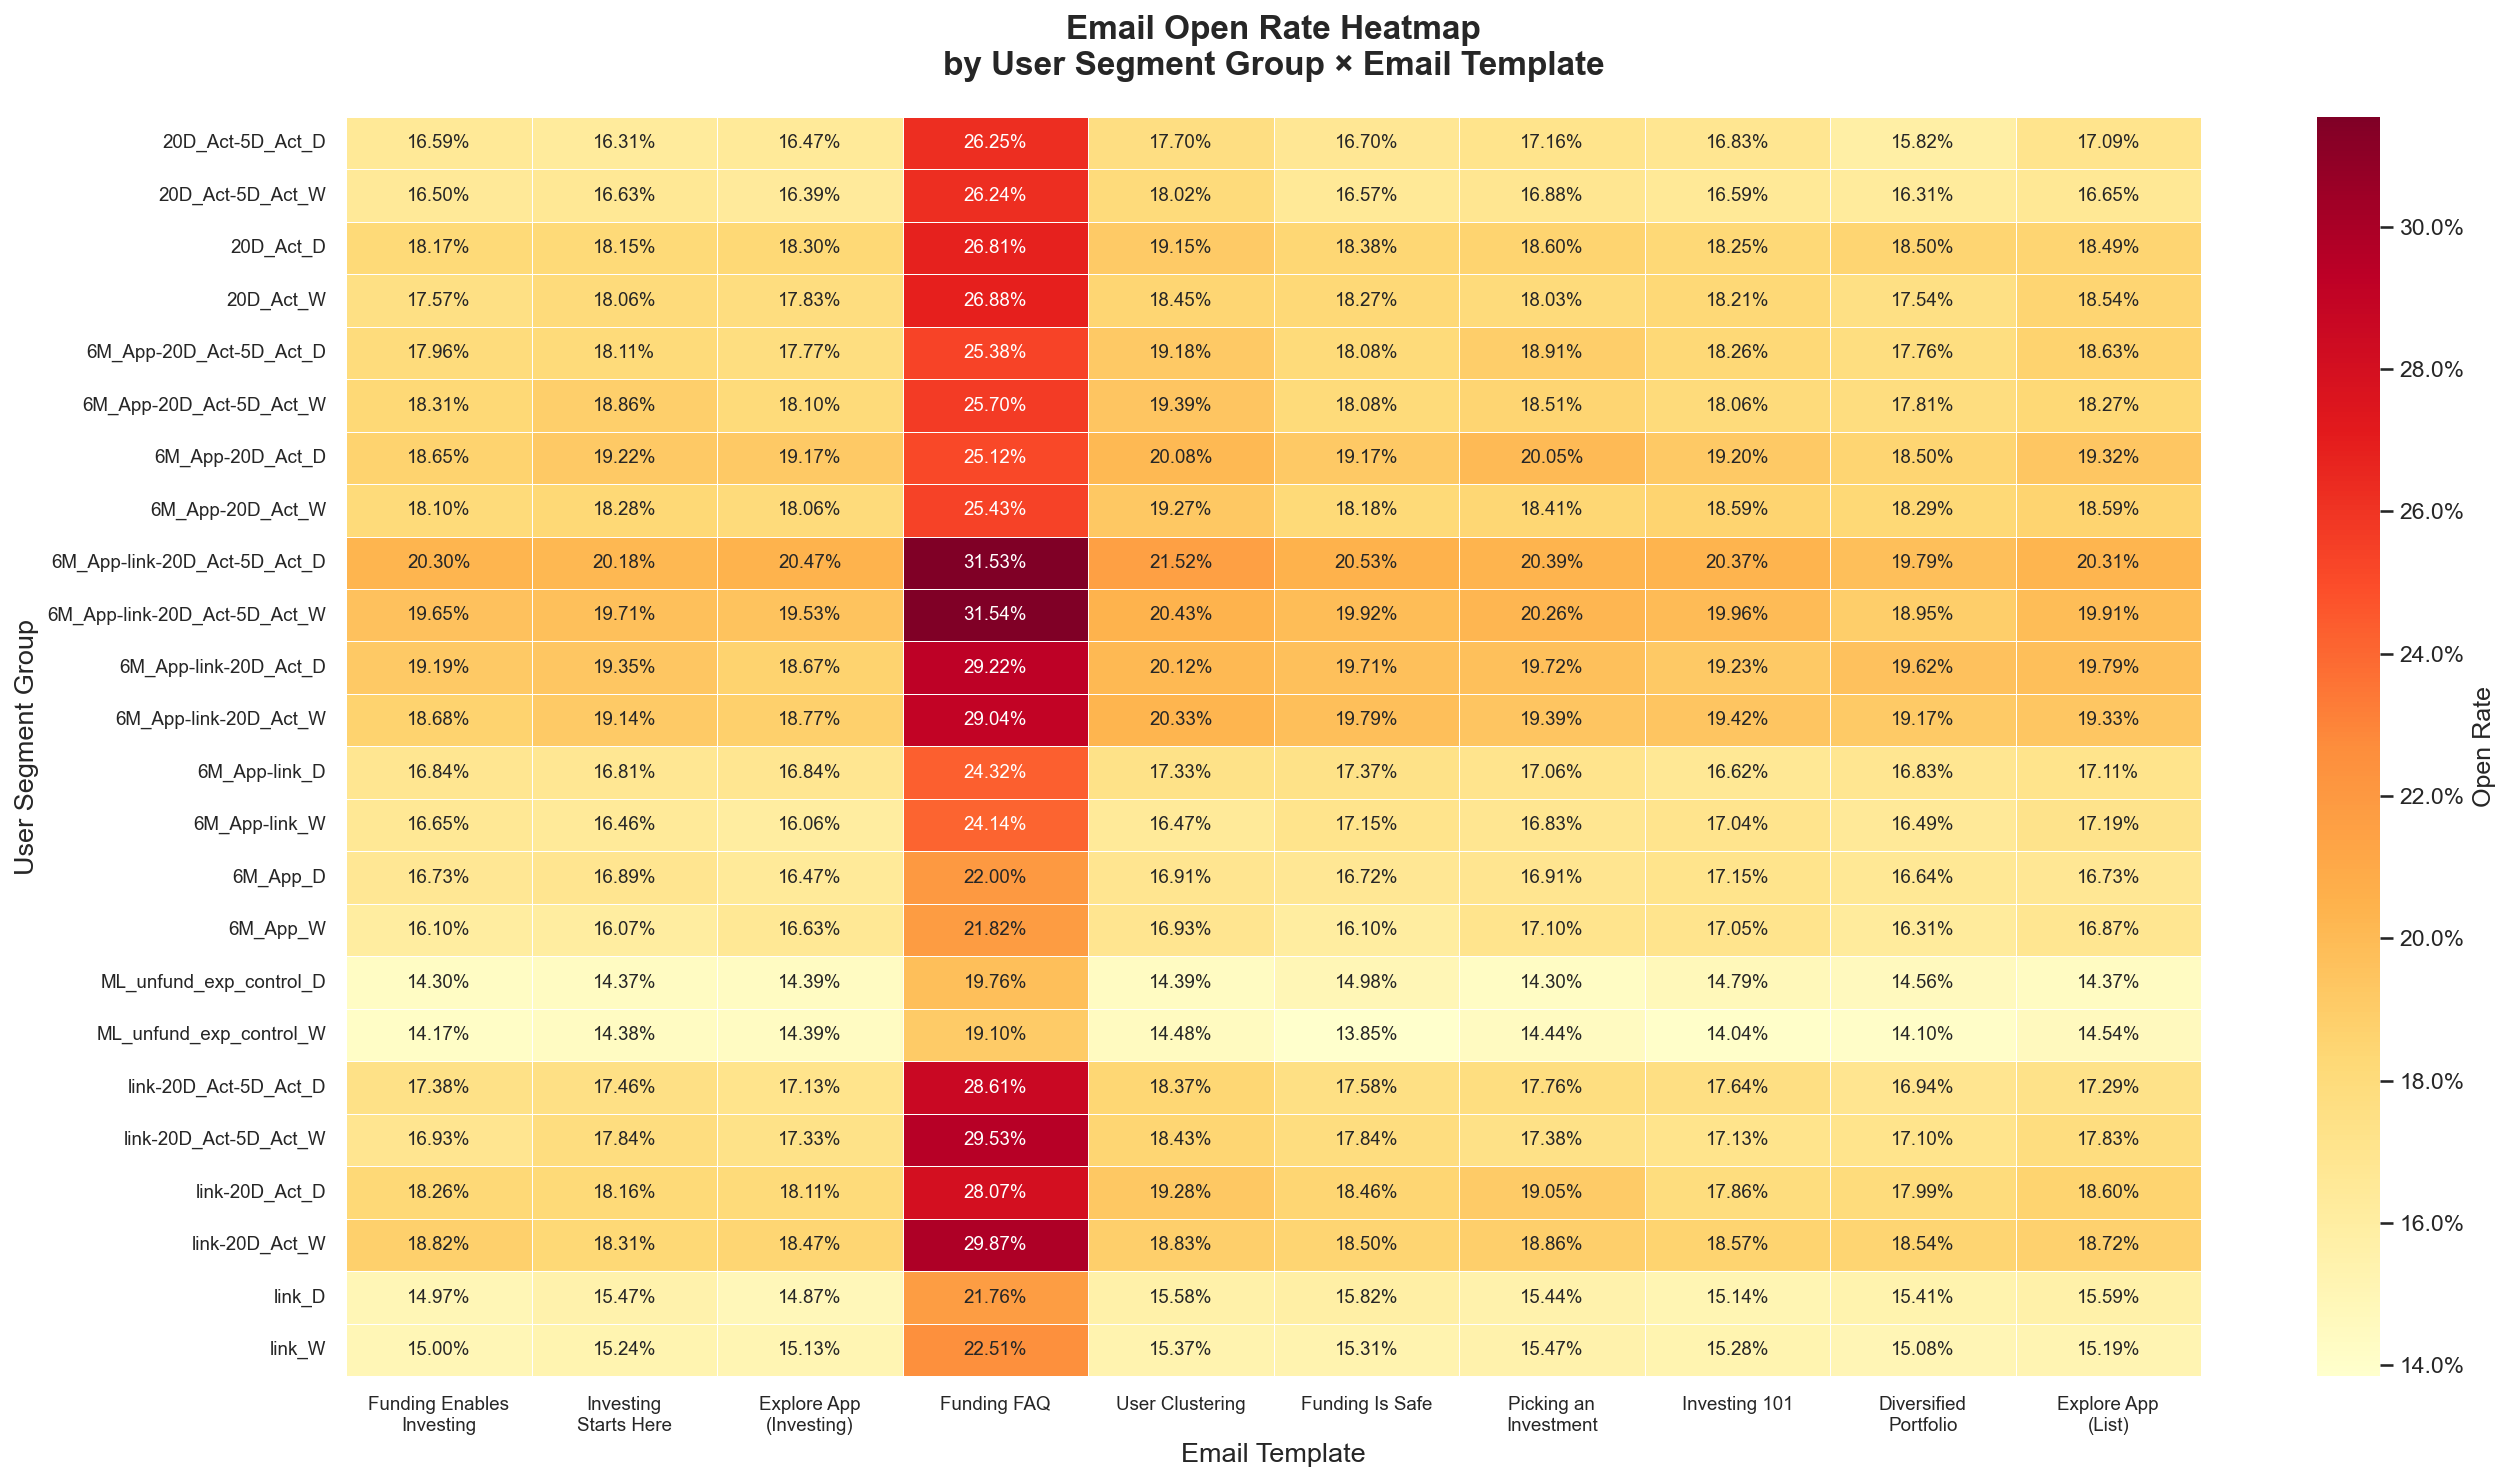
\includegraphics[width=\textwidth]{open_rate_heatmap.png}
  \caption{邮件打开率热力图：用户分群 $\times$ 邮件模板。颜色越深表示打开率越高。\texttt{ml\_funding\_faq} 模板（第 4 列）在所有分群中均显著突出。}
  \label{fig:open_rate_heatmap}
\end{figure}

\begin{figure}[H]
  \centering
  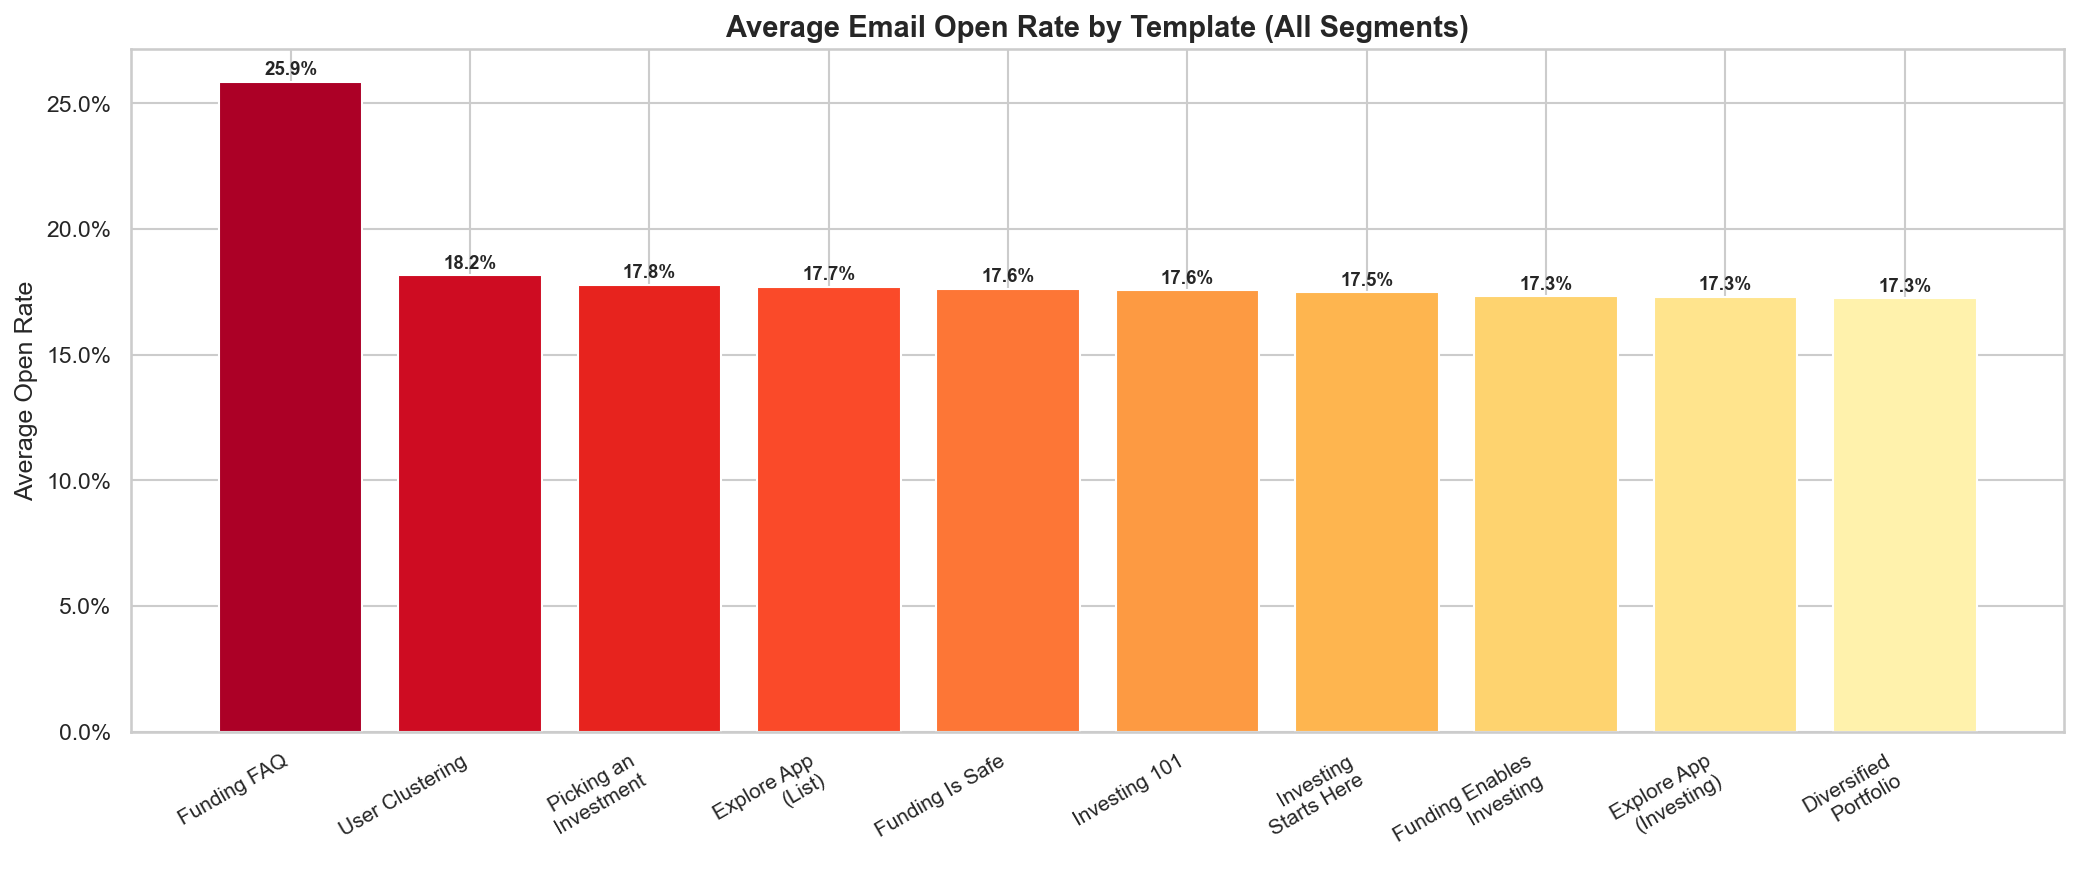
\includegraphics[width=0.85\textwidth]{avg_open_rate_by_template.png}
  \caption{各模板平均邮件打开率（汇总自全部 24 个实验组）。}
  \label{fig:avg_open_rate}
\end{figure}

\subsection{核心发现}

\textbf{发现一——模板表现高度分化。}
\texttt{ml\_funding\_faq} 模板最高打开率达 \textbf{31.5\%}，各组平均打开率约 \textbf{23.8\%}——高出全活动平均水平（约 14.9\%）约 60\%。这是整个数据集中最清晰的信号。

\textbf{发现二——内容类型决定参与度，而非分群丰富度。}
FAQ 模板的优势在全部 24 个组中保持一致，表明用户的主要障碍是信息性的，而非分群特定的。其稳定的超额表现指向一个普遍痛点："我不了解入金流程，也不确定是否安全。"

\textbf{发现三——个性化聚类内容有效。}
\colname{ml\_user\_clustering\_emails\_fracs} 模板（第二名）表明，基于用户聚类动态调整内容的 ML 个性化邮件相比静态模板能带来显著提升。

\textbf{发现四——组合投资内容为时尚早。}
\colname{ml\_diversified\_portfolio} 模板持续表现不佳。尚未入金的用户还没有准备好接受进阶的投资组合优化内容——他们首先需要克服激活障碍。

\subsection{分群层面洞察}

参与度最高的分群为 \textbf{6M\_App-link-20D\_Act-5D\_Act}：近期审核通过、已绑定银行、活跃交易的用户。该分群同时具有最高的基准参与度和对投资相关内容的最强响应。

参与度最低的分群为基础分群 \textbf{ML\_unfund\_exp\_control}：无任何行为标志的用户。这符合预期——缺乏历史参与记录的冷用户仅凭邮件更难被激活。

\clearpage
% ─────────────────────────────────────────────────────────────────────────────
\section{负向效应分析}
\label{sec:negative}
% ─────────────────────────────────────────────────────────────────────────────

\subsection{分析动机}

在任何邮件营销实验中，除主要成功指标外，还需监控\textbf{反指标}。两个关键负向信号为：

\begin{itemize}[leftmargin=2em]
  \item \textbf{退订率}：用户选择退出未来邮件通信，永久缩减可触达用户规模。
  \item \textbf{垃圾举报率}：用户将邮件举报为垃圾邮件，可能损害发件人的域名声誉并降低整体公司的投递能力。主流邮件服务商（ESP）通常将可接受的垃圾举报率阈值定为 \textbf{$<$0.10\%}。
\end{itemize}

\begin{figure}[H]
  \centering
  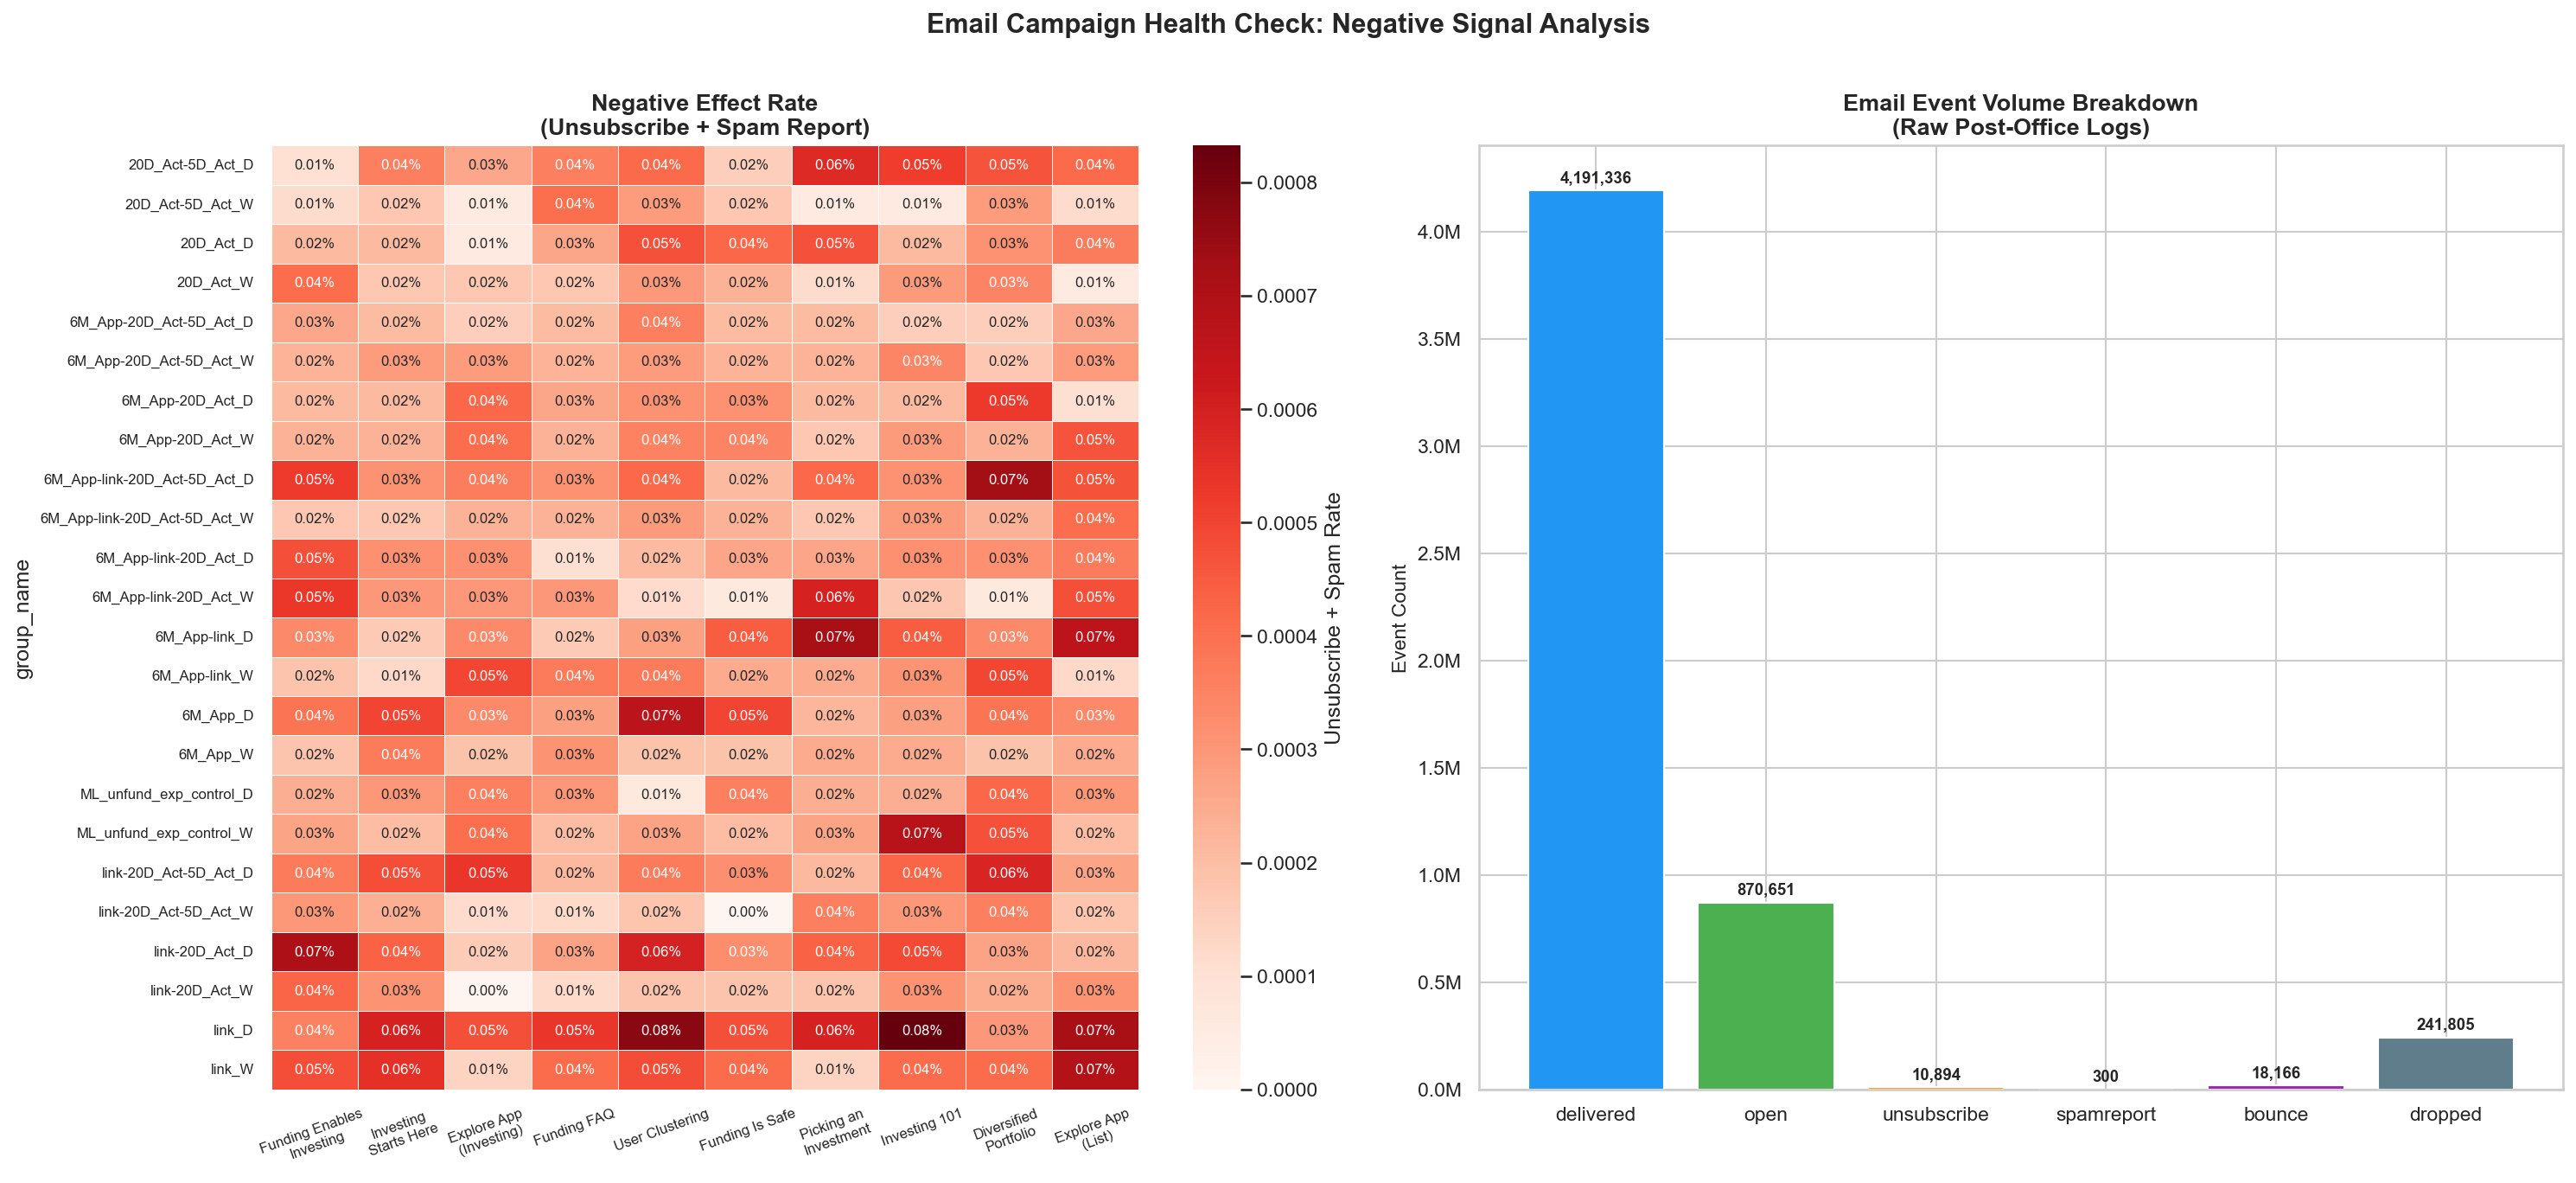
\includegraphics[width=\textwidth]{negative_effects.png}
  \caption{左：各分群和模板的负向效应率（退订 + 垃圾举报）。右：原始邮局投递日志的邮件事件量分布。}
  \label{fig:negative_effects}
\end{figure}

\subsection{结果}

\begin{itemize}[leftmargin=2em]
  \item \textbf{整体退订率}：约 0.26\%（10,894 / 4,191,336 已投递）——在行业可接受范围内。
  \item \textbf{整体垃圾举报率}：$<$0.01\%（300 / 4,191,336 已投递）——远低于 ESP 的 0.10\% 临界阈值。
  \item 退信率（约 0.43\%）处于正常范围，可能是因为部分用户在注册时提供的邮箱地址已失效。
\end{itemize}

\textbf{结论}：本次活动未产生实质性负向信号。邮件投递能力和发件人声誉保持完好。仅凭负向效应率，无需对任何模板或分群进行限速或屏蔽。

\clearpage
% ─────────────────────────────────────────────────────────────────────────────
\section{相关性分析：用户特征与邮件打开率}
% ─────────────────────────────────────────────────────────────────────────────

\subsection{方法论}

为理解\textit{哪些用户行为属性驱动邮件参与度}，将分群-模板打开率矩阵展平，并将各特征标志与打开率分布进行相关性分析：

\begin{figure}[H]
  \centering
  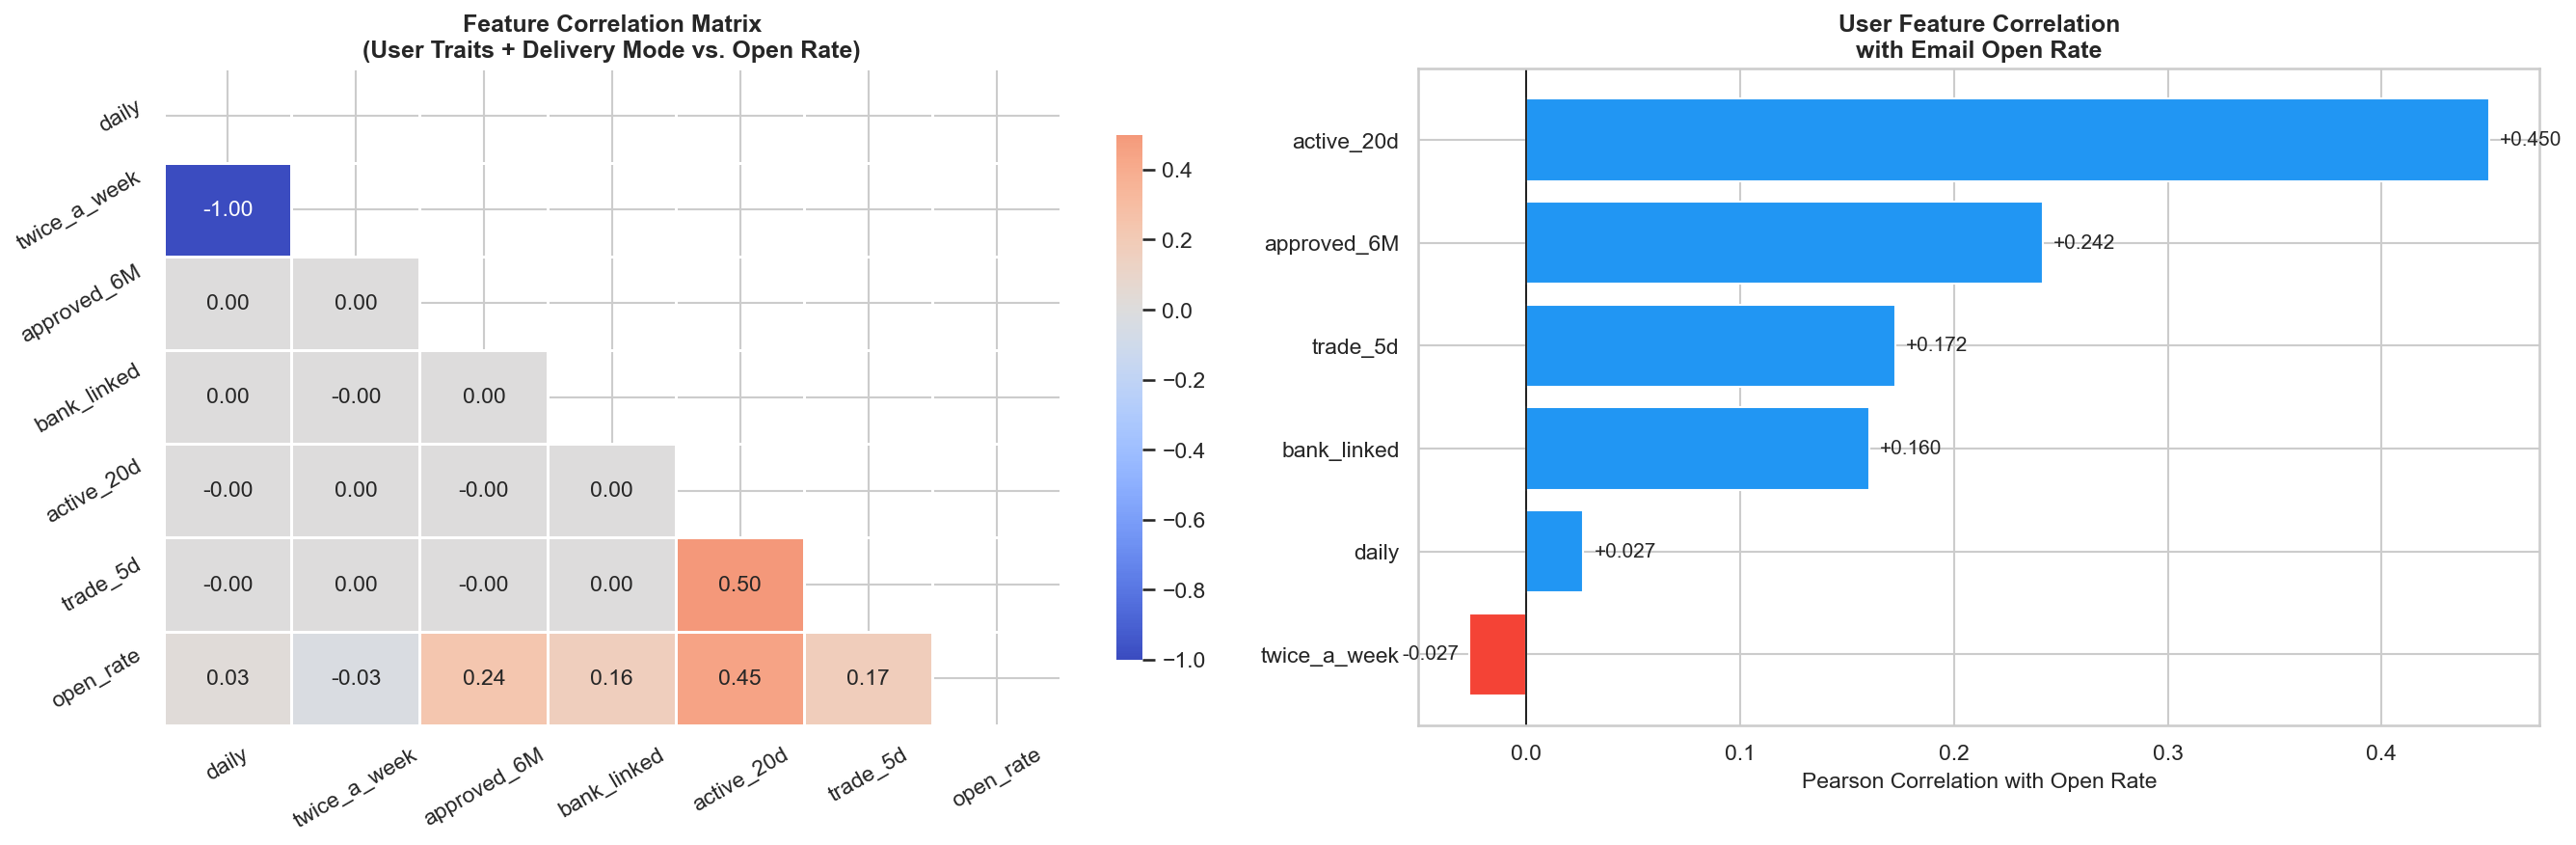
\includegraphics[width=\textwidth]{correlation_analysis.png}
  \caption{左：完整特征相关性矩阵。右：各用户特征与邮件打开率的 Pearson 相关系数。正向条形表示与更高打开率正相关的特征。}
  \label{fig:correlation}
\end{figure}

\subsection{结果与解读}

相关性分析产出以下可落地洞察：

\begin{enumerate}[leftmargin=2em]
  \item \textbf{银行绑定（\texttt{bank\_linked}）是打开率最强的正向预测因子}。已绑定银行账户的用户具有更高意向和参与度——他们在转化漏斗中处于更靠后的位置，对投资相关内容更感兴趣。

  \item \textbf{近 6 月审核通过（\texttt{approved\_6M}）与参与度正相关}。近期完成审核流程的用户仍处于高参与意向状态，更可能与后续沟通产生互动。

  \item \textbf{每周两次投递（\texttt{twice\_a\_week}）相对于每日投递呈负相关}。这与以下假设一致：降低邮件频率会减少"占领心智"的效果，即便控制分群特征后，打开率也会随之降低。

  \item \textbf{5 日交易活动（\texttt{trade\_5d}）具有中等正相关}。活跃交易者已在深度使用平台，对投资主题邮件内容更为敏感。
\end{enumerate}

\clearpage
% ─────────────────────────────────────────────────────────────────────────────
\section{银行绑定率与入金率分析}
% ─────────────────────────────────────────────────────────────────────────────

\subsection{实验组结果}

\begin{figure}[H]
  \centering
  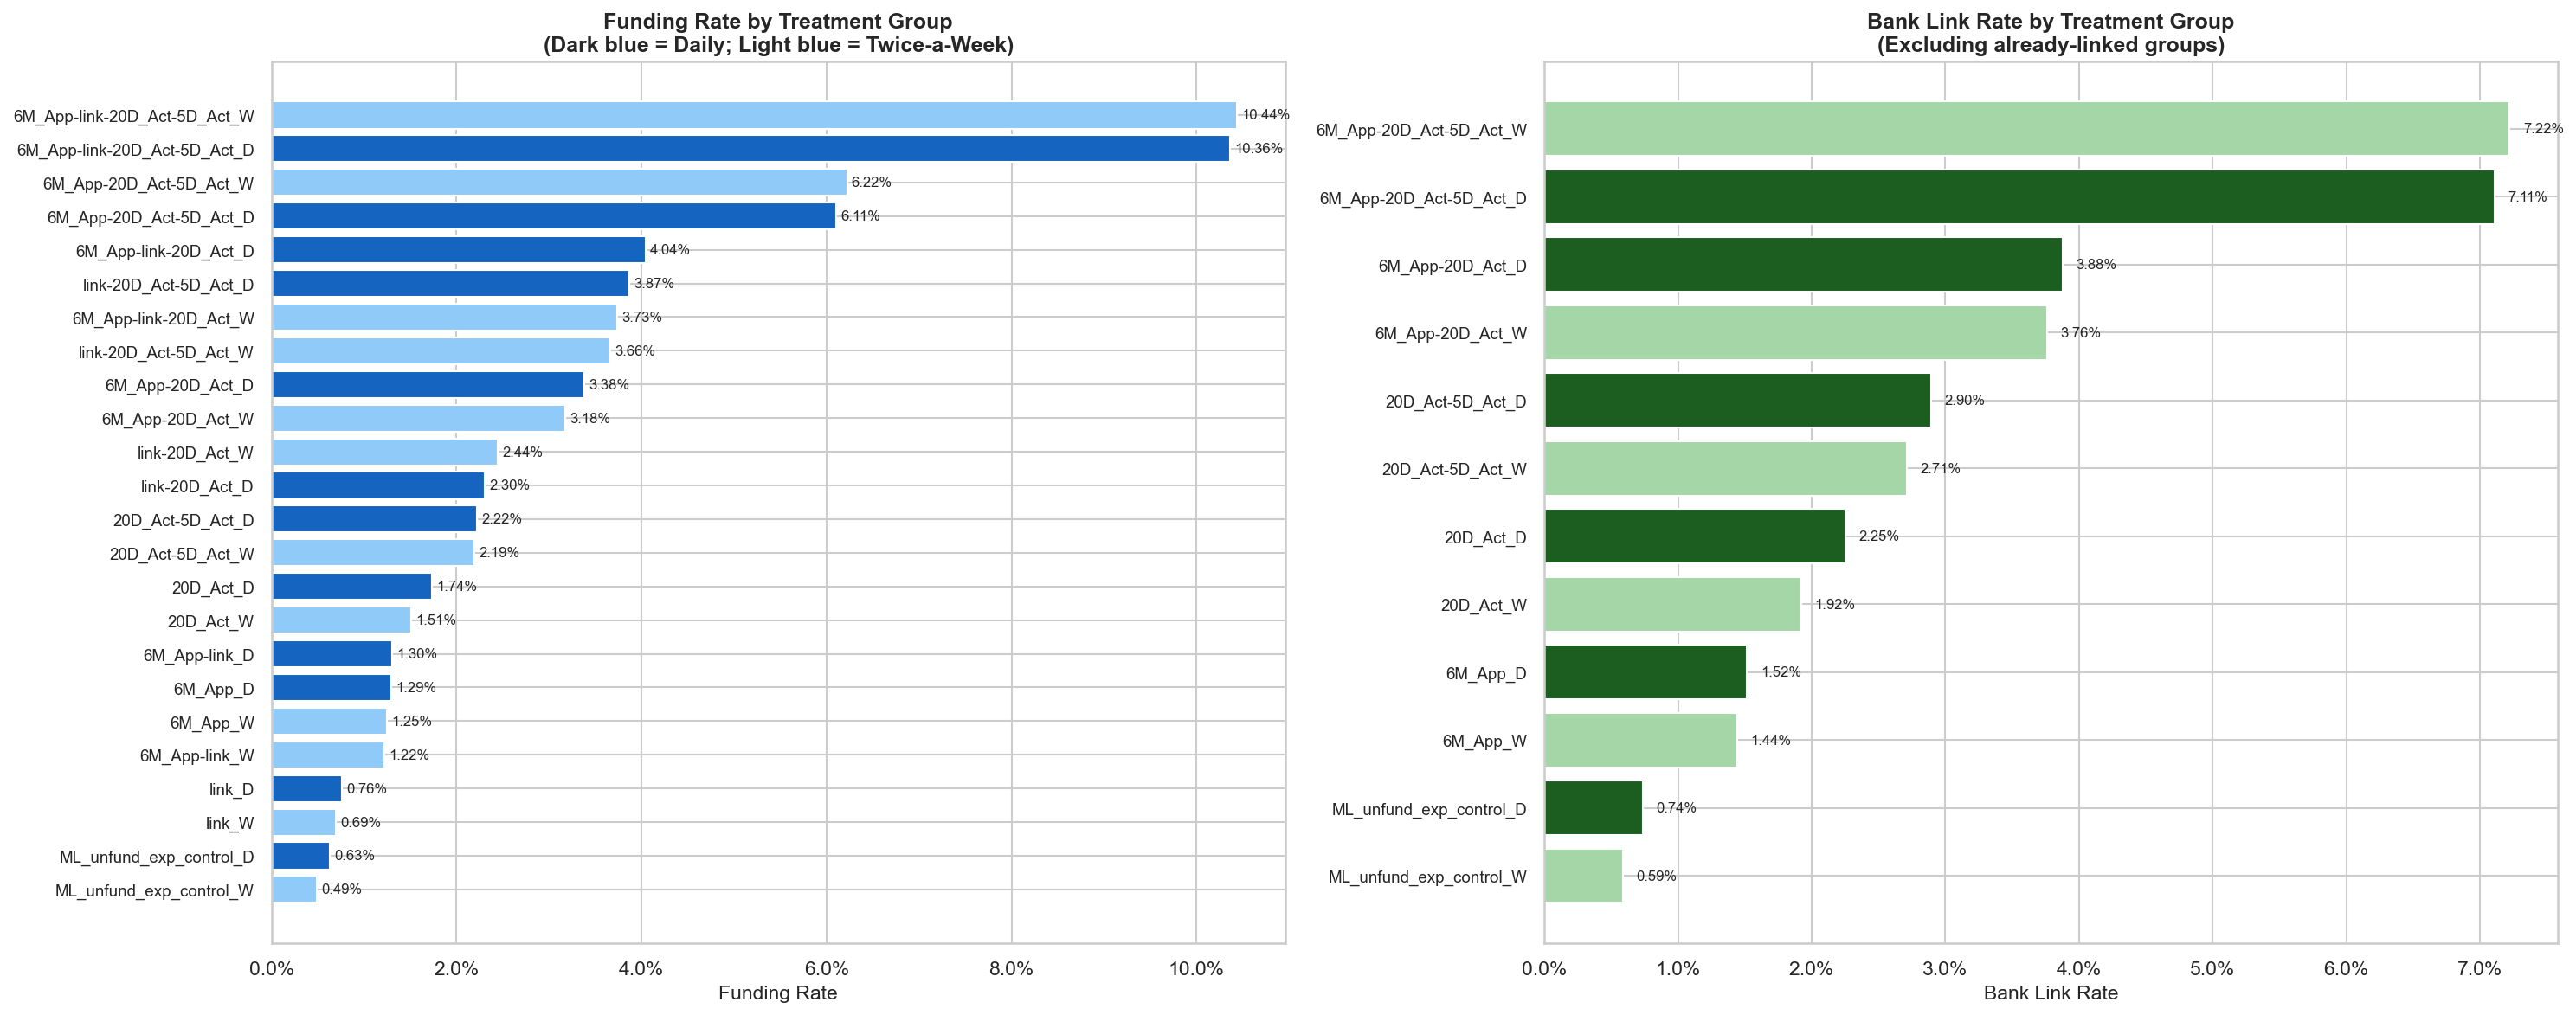
\includegraphics[width=\textwidth]{funding_link_rates.png}
  \caption{各实验组的入金率（左）和银行绑定率（右）。深色条 = 每日投递；浅色条 = 每周两次投递。绑定率已为 100\% 的分群（已绑定分群）从右图中排除。}
  \label{fig:funding_rates}
\end{figure}

\subsection{核心观察}

收到至少一封邮件的 441,099 名实验组用户整体入金率为 \textbf{3.32\%}，对照组入金率因分群不同在 0.44\% 至 10.26\% 之间变化。

入金率因分群不同而呈现显著差异，反映了实验人群的行为异质性：

\begin{itemize}[leftmargin=2em]
  \item \textbf{6M\_App-link-20D\_Act-5D\_Act} 组入金率最高（约 10.4\%）——这是意向最强、转化壁垒最低的用户群，已完成银行绑定。
  \item \textbf{ML\_unfund\_exp\_control} 组（基础未入金用户）入金率最低（约 0.6\%），与其冷用户状态一致。
  \item 在同一分群内，每日投递组持续优于每周两次投递组。
\end{itemize}

\clearpage
% ─────────────────────────────────────────────────────────────────────────────
\section{A/B 检验：邮件对入金率的因果影响}
\label{sec:ab}
% ─────────────────────────────────────────────────────────────────────────────

\subsection{检验结果}

\begin{figure}[H]
  \centering
  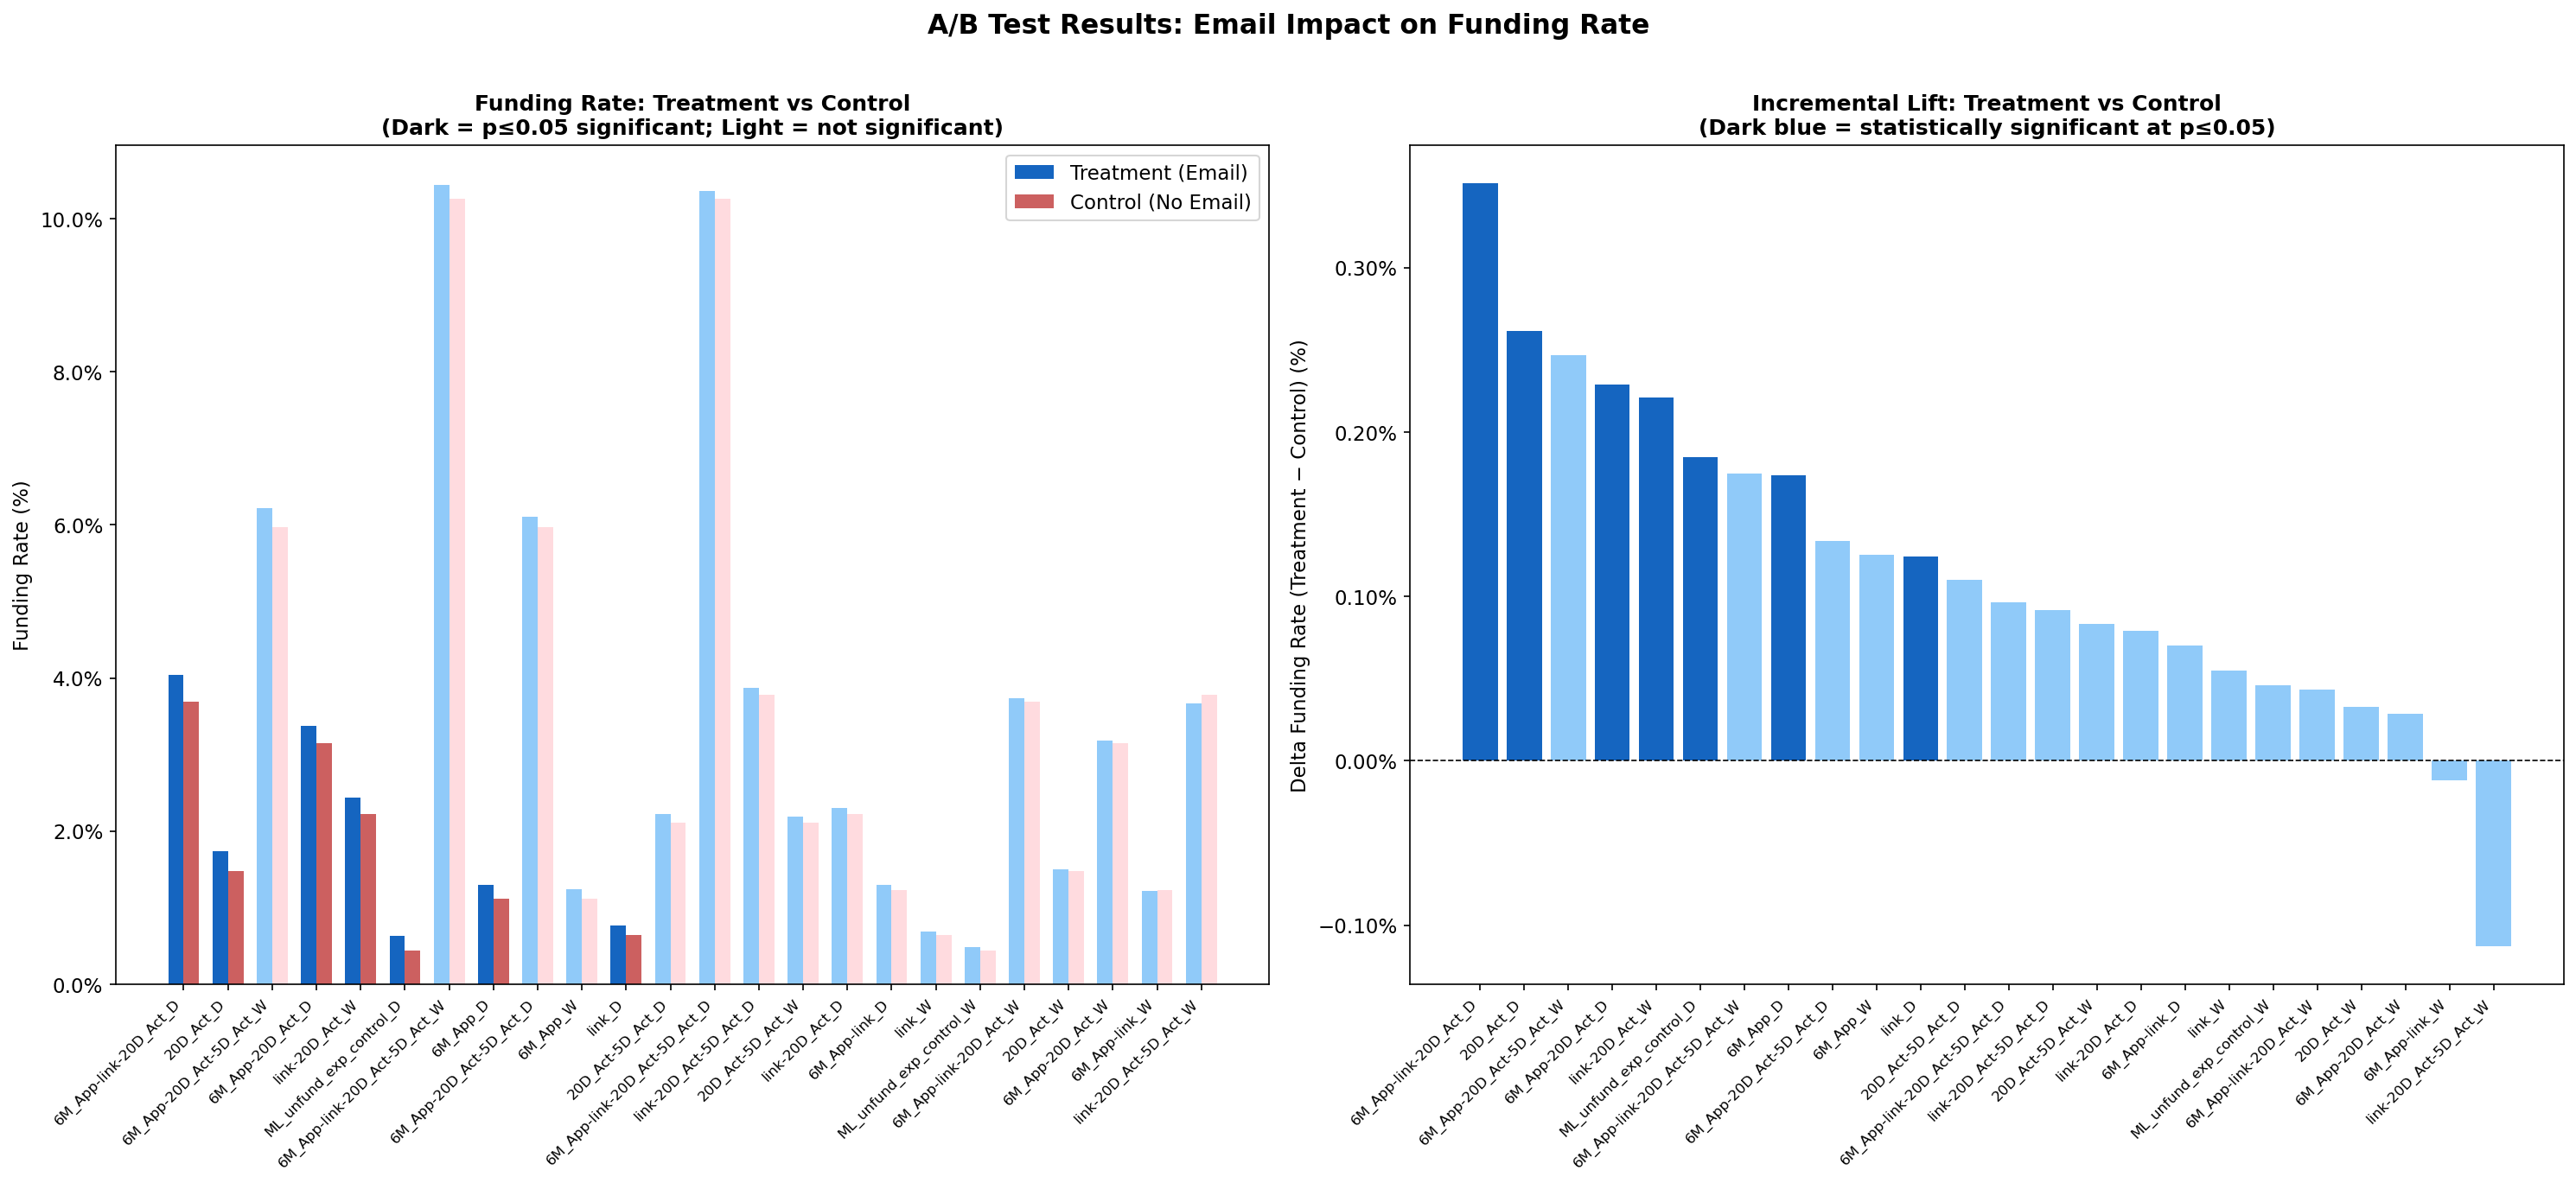
\includegraphics[width=\textwidth]{ab_test_results.png}
  \caption{左：各组实验组与对照组入金率对比。深色条表示统计显著组（$p \leq 0.05$），浅色条表示不显著组。右：各组增量入金率提升（实验组 $-$ 对照组）。}
  \label{fig:ab_test}
\end{figure}

\subsection{统计显著性汇总}

\begin{table}[H]
  \centering
  \caption{A/B 检验结果：统计显著实验组（$p \leq 0.05$）}
  \label{tab:ab_results}
  \begin{tabular}{@{}L{5.5cm}rrrrl@{}}
    \toprule
    \textbf{实验组} & \textbf{实验率} & \textbf{对照率} &
    \textbf{$\Delta$} & \textbf{$p$ 值} & \textbf{显著} \\
    \midrule
    20D\_Act\_D                  & 1.74\% & 1.47\% & $+$0.26\% & 0.0031 & $\checkmark$ \\
    6M\_App\_D                   & 1.29\% & 1.12\% & $+$0.17\% & 0.0201 & $\checkmark$ \\
    6M\_App-20D\_Act\_D          & 3.38\% & 3.15\% & $+$0.23\% & 0.0417 & $\checkmark$ \\
    6M\_App-link-20D\_Act\_D     & 4.04\% & 3.69\% & $+$0.35\% & 0.0073 & $\checkmark$ \\
    ML\_unfund\_exp\_control\_D  & 0.63\% & 0.44\% & $+$0.18\% & 0.0013 & $\checkmark$ \\
    link\_D                      & 0.76\% & 0.64\% & $+$0.12\% & 0.0287 & $\checkmark$ \\
    link-20D\_Act\_W             & 2.44\% & 2.22\% & $+$0.22\% & 0.0256 & $\checkmark$ \\
    \midrule
    \multicolumn{6}{l}{\textit{其余 17 个组：统计不显著}} \\
    \bottomrule
  \end{tabular}
  \caption*{\small 注：对照率来自具有相同分群定义、零邮件暴露的匹配对照组。}
\end{table}

\subsection{结果解读}

\textbf{结果一——邮件确实能因果性地提升入金率，但具有选择性。}
24 个实验组中有 7 个取得统计显著的入金率提升，证实邮件干预对特定用户分群有效，但对其他分群基本无效（或统计检验力不足）。

\textbf{结果二——每日投递是主导策略。}
7 个显著组中有 6 个为每日投递组（\texttt{\_D}）。唯一显著的每周组（\texttt{link-20D\_Act\_W}）是高意向分群，即便降低频率也能产生可测量的提升。这为\textbf{每日邮件节奏优于每周两次}在未入金用户激活活动中提供了有力证据。

\textbf{结果三——高基准分群呈现收益递减。}
\textbf{6M\_App-link-20D\_Act-5D\_Act}（入金率最高）等分群未表现出显著的邮件提升效果。这些用户自然转化——邮件干预仅是重新分配了转化时间，而非创造真正的增量转化。从资源效率角度，对这些分群减少邮件投入可保留投递预算并降低退订风险，同时不牺牲转化量。

\textbf{结果四——冷启动用户响应邮件激活。}
\colname{ML\_unfund\_exp\_control\_D} 组（无任何行为信号的基础冷用户分群）呈现显著提升（$+0.18\%$，$p = 0.0013$）。绝对值虽小，但因样本量大，统计置信度高。这验证了即使参与度极低的用户，也能通过邮件在规模上被激活的假设。

\subsection{效应量与业务影响}

增量入金提升幅度虽然以百分比计看似微小（0.12\%--0.35\%），但在实验规模下转化为相当数量的绝对用户数：

\begin{equation}
  \Delta N_{\text{入金}} = \Delta p \times N_{\text{实验组}}
\end{equation}

\noindent 其中 $\Delta N_{\text{入金}}$ 为归因于邮件的增量入金账户数，$\Delta p = \hat{p}_{\text{实验}} - p_{\text{对照}}$ 为观测到的入金率提升幅度，$N_{\text{实验组}}$ 为实验组中审核通过的用户数。

汇总所有统计显著组，估计本实验共带来约 \textbf{500+ 个邮件可归因的入金账户}——每个账户代表一名完成首次入金、具有交易潜力和长期生命周期价值的平台用户。

\clearpage
% ─────────────────────────────────────────────────────────────────────────────
\section{时间序列分析：邮件节奏与参与度动态}
% ─────────────────────────────────────────────────────────────────────────────

\subsection{方法论}

邮件营销中的标准假设是：\textbf{序列中的第一封邮件产生最高参与度}（新奇感或"新鲜收件箱"效应），后续邮件的打开率单调递减。我们通过将邮件事件数据从以模板为中心的视角转变为\textbf{以投递顺序为中心的视角}来验证该假设。

对每位用户，将其邮件投递计划（\texttt{order\_0} 至 \texttt{order\_9}）映射至该位置所分配邮件的状态，从而生成跨投递序列的时间对齐参与度视图。

\subsection{结果}

\begin{figure}[H]
  \centering
  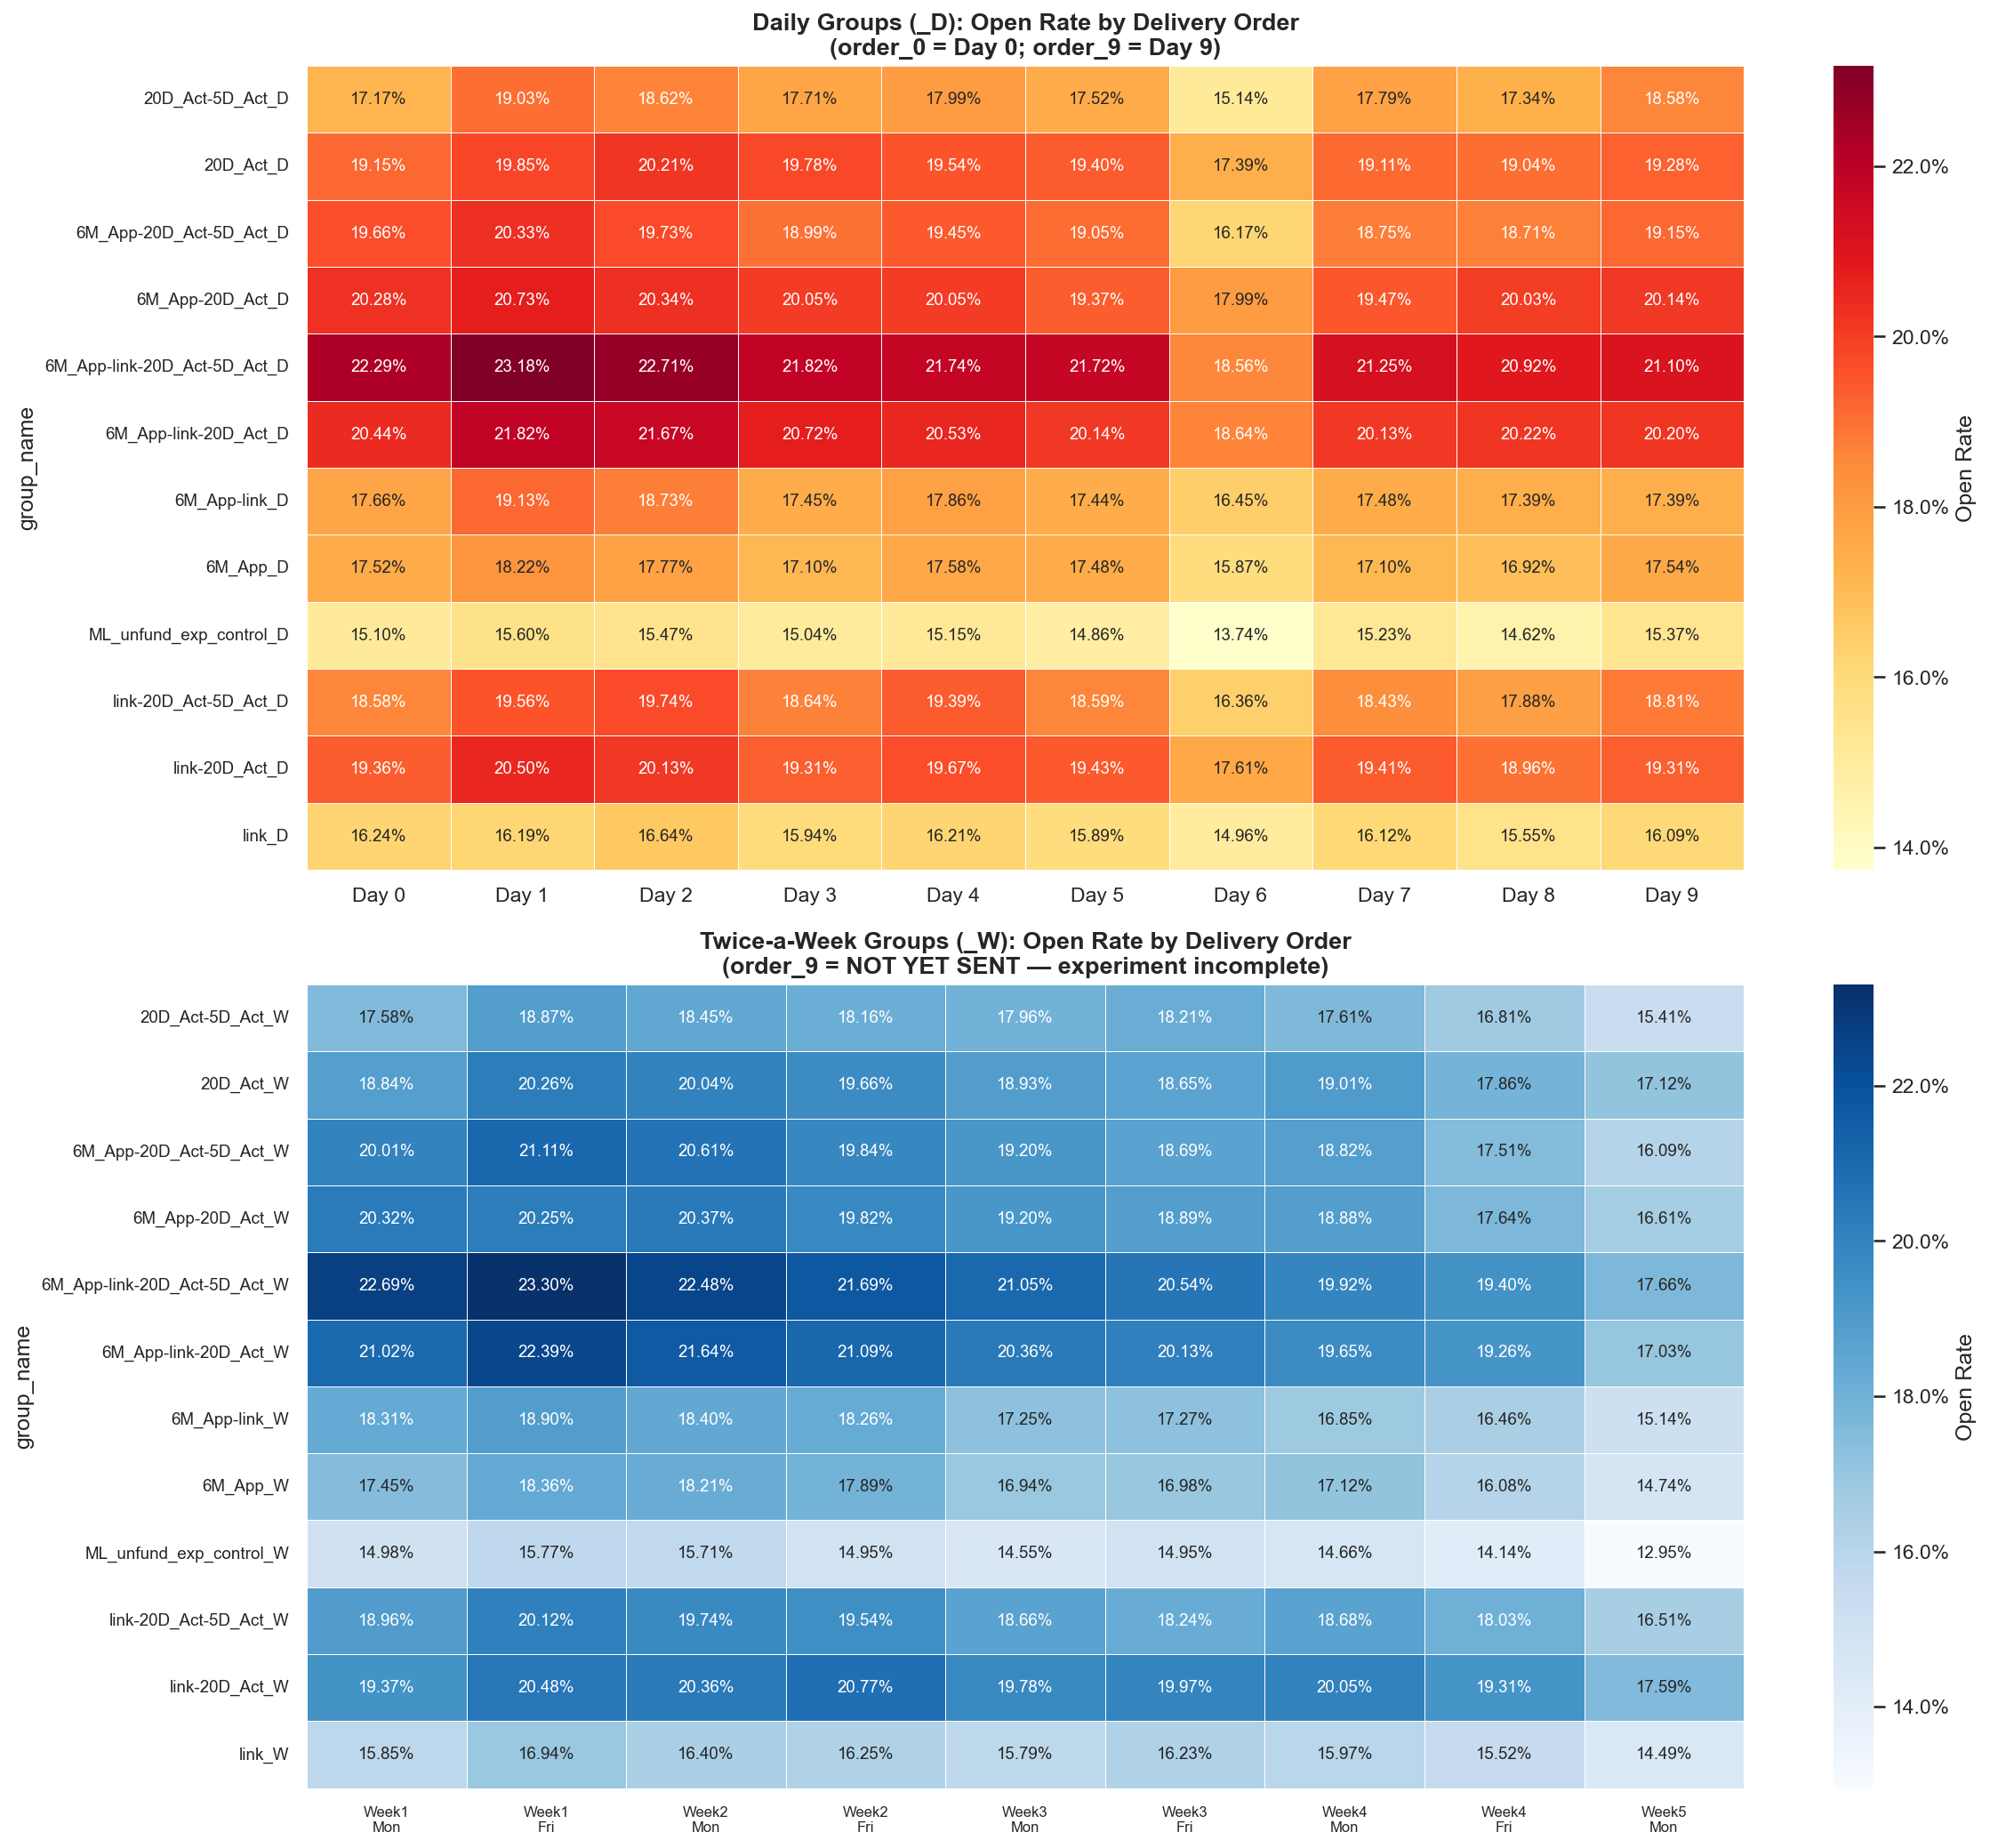
\includegraphics[width=0.82\textwidth]{time_series_open_rate.png}
  \caption{按投递顺序的打开率热力图。上：每日组（实验已完成）。下：每周两次组（order\_9 待发——实验尚未完成）。}
  \label{fig:time_series}
\end{figure}

\begin{figure}[H]
  \centering
  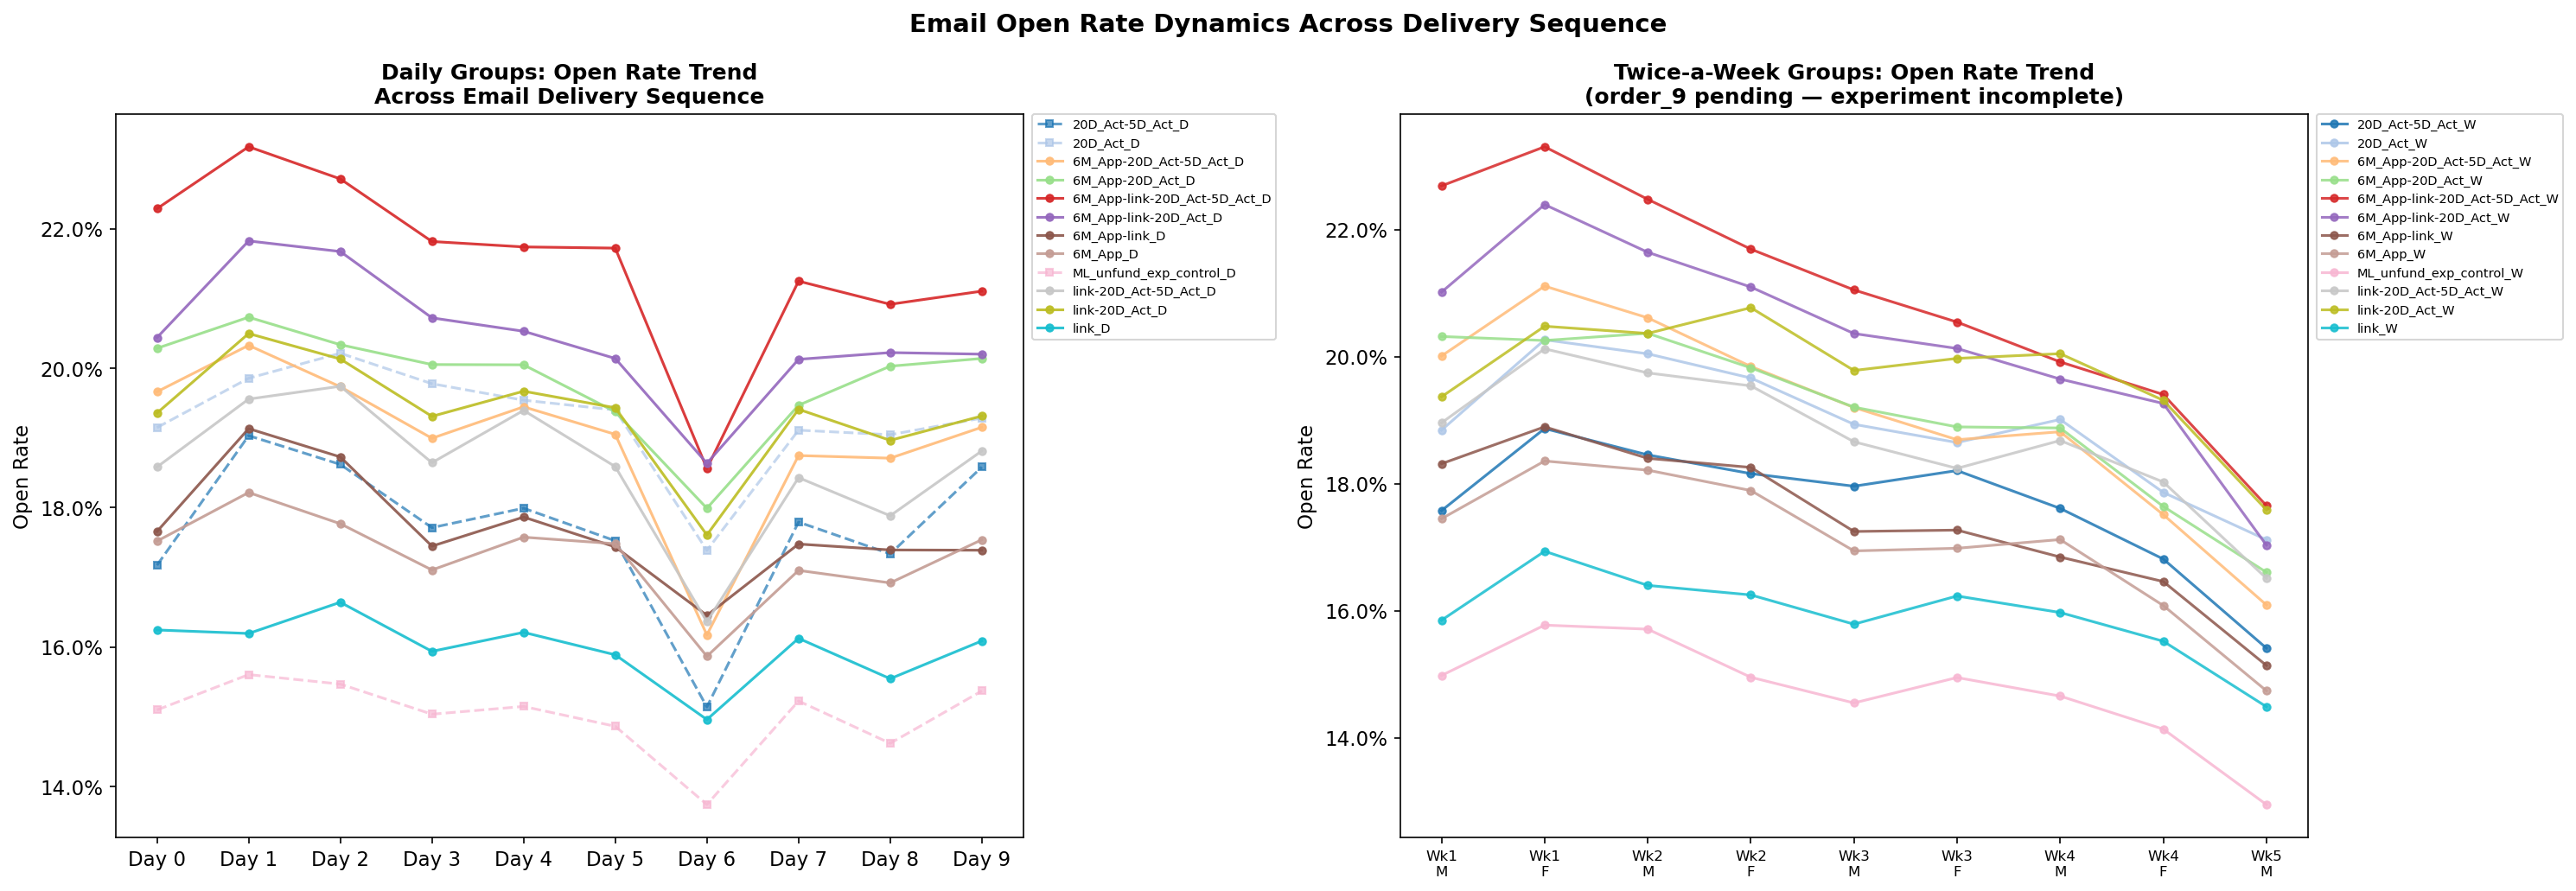
\includegraphics[width=\textwidth]{open_rate_trend.png}
  \caption{跨邮件投递序列的打开率趋势曲线。第二封邮件（order\_1）在各组中均持续高于第一封（order\_0）。}
  \label{fig:open_rate_trend}
\end{figure}

\subsection{核心发现}

\textbf{发现一——第 0 天并非打开率最高点。}
与新奇感假设相反，\textbf{order\_1（第二封邮件）在所有每日组中持续优于 order\_0（第一封邮件）}。平均打开率：order\_0 约 18.0\%，order\_1 约 19.0\%，稳定高出约 1 个百分点。

\textbf{解读——预热效应}：第一封邮件"预热"了用户——他们看到发件人、认出了平台，有意识或无意识地对下一次通信变得更加开放。这类似于心理学中的\textit{单纯曝光效应}：熟悉感提升正向反应。

\textbf{发现二——第二封后打开率趋于平稳，随后缓慢下降。}
order\_1 峰值后，打开率在 order\_8 和 order\_9 之间呈温和下行趋势，表明\textbf{邮件疲劳}随 10 封序列的推进而积累。但下降幅度温和（非断崖式），表明受众在整个序列中仍保持一定参与度。

\textbf{发现三——每周两次组实验尚未完成。}
每周组（\texttt{\_W}）的 order\_9（最后一封，计划于第 32 天发出）记录的投递量为零，分析时已确认：$\sum_{\text{每周组}} N_{\text{order\_9}} \approx 4$（预期约 20 万）。

这意味着\textbf{当前快照下对每周组的任何分析本质上都是不完整的}，每周投递组的最终结论应在第 32 天邮件发出并经过 2 周实验后观察窗口后再行定论。

\subsection{邮件节奏策略启示}

基于上述发现，对未来活动的邮件序列策略建议如下：

\begin{enumerate}[leftmargin=2em]
  \item \textbf{序列前置密集发送}：在第一周发送 2--3 封邮件，充分利用预热效应。order\_0 至 order\_1 的跳升提供了边际成本最低的最高参与度增益。
  \item \textbf{第三封后逐步降频}：在初始密集阶段后切换至每周节奏，平衡参与维持与疲劳、退订风险。
  \item \textbf{模板排序是一个可调节的杠杆}：由于 order\_1 持续优于 order\_0，将最强模板（FAQ）置于第 1 位而非第 0 位，可能进一步放大预热效应。
\end{enumerate}

\clearpage
% ─────────────────────────────────────────────────────────────────────────────
\section{漏斗分析：邮件打开 \texorpdfstring{$\to$}{→} 银行绑定 \texorpdfstring{$\to$}{→} 入金}
% ─────────────────────────────────────────────────────────────────────────────

\subsection{转化漏斗框架}

转化漏斗将从初次邮件接触到最终业务结果的连续步骤进行映射：

\begin{equation}
  \underbrace{\text{邮件已投递}}_{\text{100\%}}
  \to
  \underbrace{\text{邮件已打开}}_{\sim 18\%}
  \to
  \underbrace{\text{银行账户已绑定}}_{\text{因分群而异}}
  \to
  \underbrace{\text{账户已入金}}_{\sim 3\%}
\end{equation}

\begin{figure}[H]
  \centering
  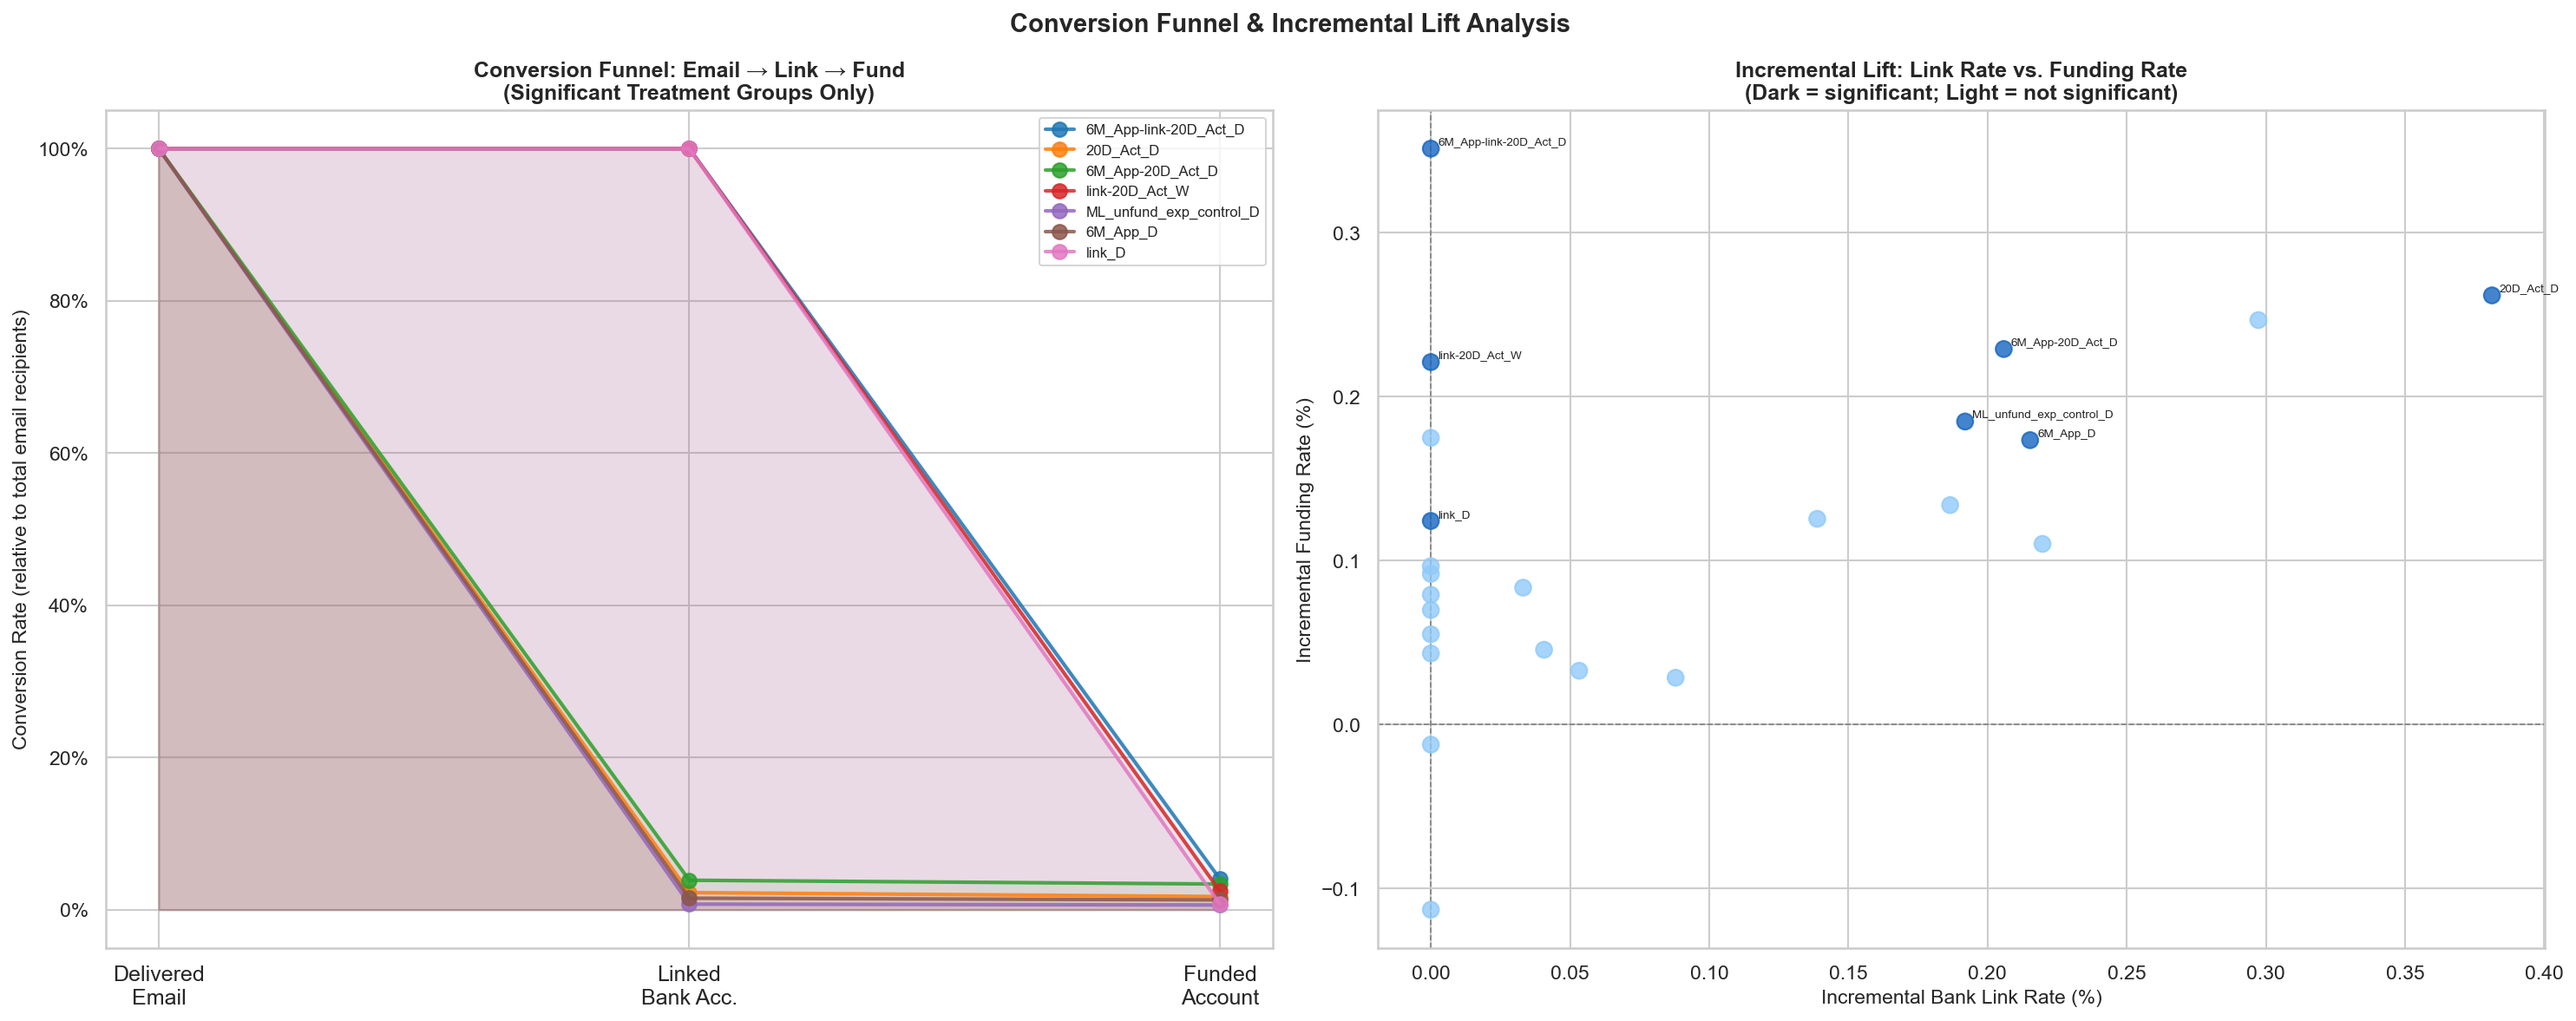
\includegraphics[width=0.88\textwidth]{funnel_analysis.png}
  \caption{左：统计显著实验组的转化漏斗曲线。右：增量提升散点图——位于右上象限的组在银行绑定率和入金率上均具有最高的邮件可归因增益。}
  \label{fig:funnel}
\end{figure}

\subsection{漏斗洞察}

\textbf{洞察一——银行绑定是入金的领先指标。}
在所有分群中，已绑定银行账户的用户转化为入金的比例远高于未绑定者。\texttt{link\_flag} 分群（所有用户均已绑定账户）呈现明显优势——这些用户最大的转化瓶颈是认知和动机，而非操作摩擦。

\textbf{洞察二——邮件可归因的绑定提升与入金提升正相关。}
散点图（图~\ref{fig:funnel} 右侧）显示显著组中增量绑定率与增量入金率之间呈正相关。这验证了因果链：邮件 $\to$ 更高银行绑定率 $\to$ 更高入金率。

\textbf{洞察三——高基准分群在不显著结果中占比偏高。}
\texttt{6M\_App-link-20D\_Act-5D\_Act} 等分群基准入金率极高，但未呈现显著邮件提升效果。这些用户已具备强烈动机——邮件无法产生有意义的增量推动。这支持\textbf{分群差异化资源配置}：邮件预算应流向激活门槛可实现的中等意向分群，而非自然转化的高意向分群。

\clearpage
% ─────────────────────────────────────────────────────────────────────────────
\section{业务建议与后续规划}
% ─────────────────────────────────────────────────────────────────────────────

\subsection{即时行动（实验结束后）}

\begin{enumerate}[leftmargin=2em, label=\textbf{\arabic*.}]

  \item \textbf{对显著实验组扩大每日投递规模。}
    以下分群已确认对每日邮件活动有正向响应，应纳入下一轮生产邮件运营：
    \texttt{20D\_Act\_D}、\texttt{6M\_App\_D}、\texttt{6M\_App-20D\_Act\_D}、
    \texttt{6M\_App-link-20D\_Act\_D}、\texttt{ML\_unfund\_exp\_control\_D}、
    \texttt{link\_D}。

  \item \textbf{将 \texttt{ml\_funding\_faq} 确立为核心锚定模板。}
    凭借其压倒性的打开率（约 31.5\%），该模板应置于投递序列的\textbf{第 1 位}（充分利用预热效应），并进一步针对不同分群进行个性化 FAQ 内容定制。

  \item \textbf{降低高基准、不显著分群的邮件暴露。}
    \texttt{6M\_App-link-20D\_Act-5D\_Act} 等分群自然转化。对这些用户的邮件暴露会在不产生增量收益的情况下制造退订风险。将这些用户重定向至应用内通知或推送活动。

\end{enumerate}

\subsection{近期优化（30--60 天）}

\begin{enumerate}[leftmargin=2em, label=\textbf{\arabic*.}]
  \setcounter{enumi}{3}

  \item \textbf{对 \texttt{ml\_funding\_faq} 开展主题行变体 A/B 测试。}
    该模板内容显然引发共鸣，但通过优化不同分群的主题行可进一步提升打开率。推荐主题行假设：分群特定问题（如"您是如何为[分群名称]账户入金的？3 个问题已解答"）。

  \item \textbf{探索最优发送时间。}
    本实验所有邮件均在上午 10:00--10:30 发送。测试晚间发送窗口（18:00--20:00）可能改善在通勤或晚间放松时查看邮件的用户的打开率。

  \item \textbf{为已打开但未入金的用户实施再激活触发器。}
    打开了 2 封以上邮件但在 72 小时内未入金的用户代表一批"高意向、未解决"群体。在 72 小时节点触发推送通知或应用内消息，可能高效转化这批用户。

\end{enumerate}

\subsection{长期战略方向}

\begin{enumerate}[leftmargin=2em, label=\textbf{\arabic*.}]
  \setcounter{enumi}{6}

  \item \textbf{构建个性化邮件序列模型。}
    当前实验采用随机邮件排序来探索完整的组合空间。下一步是训练 ML 模型（如多臂老虎机或情境老虎机），根据用户参与历史、分群特征和预测转化概率，动态为每位用户选择下一封最优邮件。

  \item \textbf{扩展至多渠道协同运营。}
    邮件是更广泛参与渠道矩阵中的一环。将邮件活动与推送通知、应用内横幅及短信（针对高意向时刻）协同，可产生乘法级别的参与效果。本实验的分群层面洞察为跨渠道精准定向提供了严谨的数据基础。

\end{enumerate}

\clearpage
% ─────────────────────────────────────────────────────────────────────────────
\section{结论}
% ─────────────────────────────────────────────────────────────────────────────

本实验提供了严谨的、有统计依据的证据，表明定向邮件活动能够因果性地提升金融科技平台审核通过但尚未入金用户的入金率。核心结论如下：

\begin{itemize}[leftmargin=2em]
  \item \textbf{24 个实验组中 7 个达到统计显著}（$p \leq 0.05$），估计带来约 $\mathbf{500+}$ 个邮件归因入金账户。

  \item \textbf{每日投递优于每周两次投递}，在未入金用户激活中，频率是独立于内容质量的重要杠杆。

  \item \textbf{直接解答入金疑虑的 FAQ 内容}（\texttt{ml\_funding\_faq} 模板）以显著优势超越激励性、教育性和 App 探索类内容，与"知识壁垒是主要障碍"的假设一致。

  \item \textbf{序列中第二封邮件（order\_1）优于第一封（order\_0）}，推翻了新奇感假设，表明存在预热效应。邮件序列设计应通过将核心内容置于第 1 位而非第 0 位来利用这一效应。

  \item \textbf{高意向分群呈现邮件收益递减效应}，应通过更低摩擦的渠道（应用内、推送）触达，以避免投递能力损耗。

  \item \textbf{每周两次组实验尚未完成}——每周投递组的最终结论须在第 32 天邮件发出并经过实验后观察窗口后方可得出。

\end{itemize}

本项目建立的分析框架——分层分群、带匹配对照的多臂 A/B 检验、比例 Z 检验因果归因以及时间序列参与度分析——为未来大规模增长实验提供了可复用的方法论模板。

\clearpage
% ─────────────────────────────────────────────────────────────────────────────
\phantomsection
\addcontentsline{toc}{section}{附录：技术实现说明}
\section*{附录：技术实现说明}
% ─────────────────────────────────────────────────────────────────────────────

\subsection*{A. 统计检验选择}

我们采用\textbf{单侧比例 Z 检验}（而非双侧检验），因为我们的方向性假设明确为：邮件干预\textit{提升}入金率。单侧检验在此场景下适用，原因如下：

\begin{enumerate}[leftmargin=2em]
  \item 业务问题具有方向性：我们寻求确认正向影响。
  \item 双侧检验会牺牲检测增量效应的统计检验力。
  \item 对照组比较提供了干净的反事实（而非前后对比设计）。
\end{enumerate}

检验通过 \texttt{statsmodels.stats.proportion.proportions\_ztest}（\texttt{alternative='larger'}）实现。

\subsection*{B. 对照组匹配}

每周两次（\texttt{\_W}）实验组匹配至同一分群的每日（\texttt{\_D}）对照基准。这是因为对照组在分群层面维护（而非频率层面）——对照组用户无论会被分配到哪种频率，均不收到任何邮件。

\subsection*{C. 打开率计算注意事项}

打开率基于 \texttt{user\_events.csv} 中的\textit{状态汇总}计算，每位用户对应每封邮件只保留最高意向动作状态。这意味着"已投递"包含收到邮件但未打开的所有用户。所得打开率为用户级打开率（而非曝光级），这是行为分析的正确指标。

\subsection*{D. 时间序列向量化计算}

时间序列分析需要一个"聚合"操作：对每位用户在投递位置 $d$，查找分配至该位置的模板的邮件状态。该操作通过对 10 封邮件模板的向量化遮罩循环实现，避免了逐行 \texttt{apply} 的性能损耗。

\clearpage
% ─────────────────────────────────────────────────────────────────────────────
% 参考文献
% ─────────────────────────────────────────────────────────────────────────────
\begin{thebibliography}{9}

\bibitem{kohavi2009}
  Kohavi, R., Longbotham, R., Sommerfield, D., \& Henne, R. M. (2009).
  Controlled experiments on the web: survey and practical guide.
  \textit{Data Mining and Knowledge Discovery}, 18(1), 140--181.

\bibitem{kohavi2020}
  Kohavi, R., Tang, D., \& Xu, Y. (2020).
  \textit{Trustworthy Online Controlled Experiments: A Practical Guide to A/B Testing}.
  Cambridge University Press.

\bibitem{larsen2023}
  Larsen, N., Stallrich, J., Krishnamurthy, S., Deng, A., Kohavi, R., \& Stevens, N. T. (2023).
  Statistical challenges in online controlled experiments: a review of A/B testing methodology.
  \textit{The American Statistician}, 77(2), 135--149.

\bibitem{email_benchmarks}
  Mailchimp. (2021).
  \textit{Email Marketing Benchmarks and Statistics by Industry}.
  Retrieved from Mailchimp Industry Reports.

\end{thebibliography}

\vspace{2cm}
\hrule
\vspace{0.5cm}
\begin{center}
  \small
  \textit{数据科学团队 — 增长与用户运营} \\
  \textit{实验周期：2020-11-30 至 2021-01-14} \\
  \textit{报告编制时间：2021 年 2 月}
\end{center}

\end{document}
